\documentclass{article}

% packages
\usepackage{amsmath, amsthm, thmtools, amsfonts, amssymb, luacode, catchfile, tikzducks, hyperref, ifthen}
\ifcsname c@kobocompile\endcsname
	\usepackage[a5paper, total={1072pt, 1448pt}, margin=10pt, includeheadfoot]{geometry} % set page margins
\else
	\usepackage[a4paper, margin=50pt, includeheadfoot]{geometry}
\fi
\usepackage[shortlabels]{enumitem}
\usepackage[skip=3pt, indent=0pt]{parskip}

% language
\usepackage[bidi=basic, layout=tabular, provide=*]{babel}
\ifcsname c@english\endcsname
	\babelprovide[main, import]{english}
\else
	\babelprovide[main, import]{hebrew}
	\babelprovide{rl}
\fi
%\babelfont{rm}{Libertinus Serif}
\babelfont{rm}[Renderer=Harfbuzz]{Libertinus Serif}
\babelfont{sf}{Libertinus Sans}
\babelfont{tt}{Libertinus Mono}

% style
\AddToHook{cmd/section/before}{\clearpage}	% Add line break before section
\linespread{1.3}
\setcounter{secnumdepth}{0}		% Remove default number tags from sections, this won't do well with theorems
\AtBeginDocument{\setlength{\belowdisplayskip}{3pt}}
\AtBeginDocument{\setlength{\abovedisplayskip}{3pt}}
\graphicspath{ {../images/} }

% operators
\DeclareMathOperator\cis{cis}
\DeclareMathOperator\Sp{Sp}
\DeclareMathOperator\tr{tr}
\DeclareMathOperator\im{Im}
\DeclareMathOperator\re{Re}
\DeclareMathOperator\diag{diag}
\DeclareMathOperator*\lowlim{\underline{lim}}
\DeclareMathOperator*\uplim{\overline{lim}}
\DeclareMathOperator\rng{rng}
\DeclareMathOperator\Sym{Sym}
\DeclareMathOperator\Arg{Arg}
\DeclareMathOperator\Log{Log}
\DeclareMathOperator\dom{dom}
\DeclareMathOperator\supp{Supp}
\DeclareMathOperator\var{Var}
\DeclareMathOperator\cov{Cov}

% commands
%\renewcommand\qedsymbol{\textbf{מש''ל}}
%\renewcommand\qedsymbol{\fbox{\emoji{lizard}}}
\newcommand{\Aa}[0]{\mathcal{A}}
\newcommand{\Bb}[0]{\mathcal{B}}
\newcommand{\CC}[0]{\mathbb{C}}
\newcommand{\Cc}[0]{\mathcal{C}}
\newcommand{\EE}[0]{\mathbb{E}}
\newcommand{\FF}[0]{\mathbb{F}}
\newcommand{\Ff}[0]{\mathcal{F}}
\newcommand{\Ii}[0]{\mathcal{I}}
\newcommand{\Gg}[0]{\mathcal{G}}
\newcommand{\Ll}[0]{\mathcal{L}}
\newcommand{\Mm}[0]{\mathcal{M}}
\newcommand{\NN}[0]{\mathbb{N}}
\newcommand{\Nn}[0]{\mathcal{N}}
\newcommand{\PP}[0]{\mathbb{P}}
\newcommand{\Pp}[0]{\mathcal{P}}
\newcommand{\QQ}[0]{\mathbb{Q}}
\newcommand{\RR}[0]{\mathbb{R}}
\newcommand{\Rr}[0]{\mathcal{R}}
\newcommand{\Ss}[0]{\mathcal{S}}
\newcommand{\TT}[0]{\mathbb{T}}
\newcommand{\Uu}[0]{\mathcal{U}}
\newcommand{\Vv}[0]{\mathcal{V}}
\newcommand{\Ww}[0]{\mathcal{W}}
\newcommand{\ZZ}[0]{\mathbb{Z}}
\newcommand{\acts}[0]{\circlearrowright}
\newcommand{\explain}[2] {
	\begin{flalign*}
		 && \text{#2} && \text{#1}
	\end{flalign*}
}
\newcommand{\maketitleprint}[0]{ \begin{center}
	%\begin{tikzpicture}[scale=3]
	%	\duck[graduate=gray!20!black, tassel=red!70!black]
	%\end{tikzpicture}	
	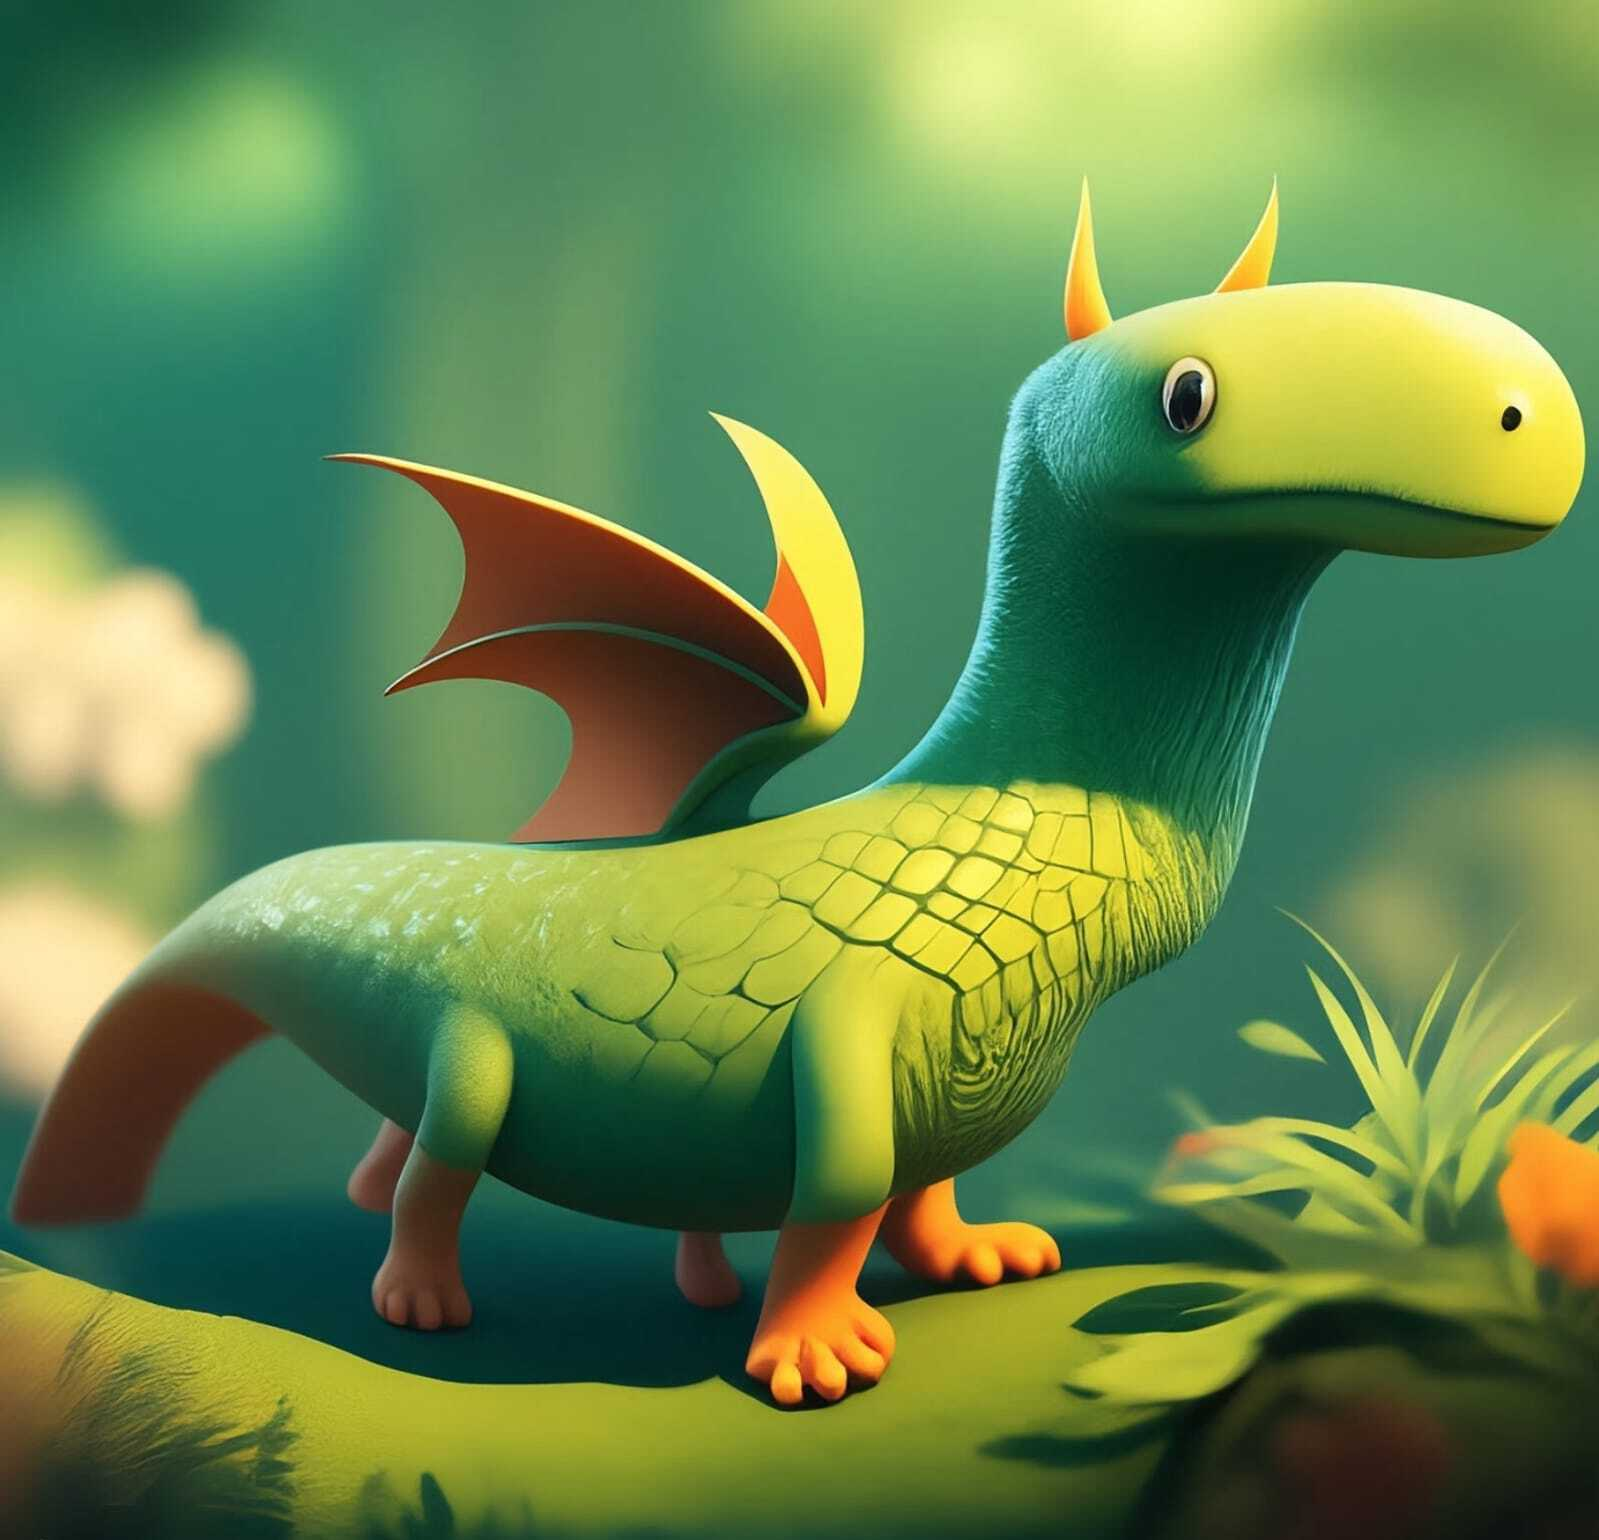
\includegraphics[width=6cm]{cover}
\end{center}
}

% theorem commands
\newtheoremstyle{c_remark}
	{}	% Space above
	{}	% Space below
	{}% Body font
	{}	% Indent amount
	{\bfseries}	% Theorem head font
	{}	% Punctuation after theorem head
	{.5em}	% Space after theorem head
	{\thmname{#1}\thmnumber{ #2}\thmnote{ \normalfont{\text{(#3)}}}}	% head content
\newtheoremstyle{c_definition}
	{3pt}	% Space above
	{3pt}	% Space below
	{}% Body font
	{}	% Indent amount
	{\bfseries}	% Theorem head font
	{}	% Punctuation after theorem head
	{.5em}	% Space after theorem head
	{\thmname{#1}\thmnumber{ #2}\thmnote{ \normalfont{\text{(#3)}}}}	% head content
\newtheoremstyle{c_plain}
	{3pt}	% Space above
	{3pt}	% Space below
	{\itshape}% Body font
	{}	% Indent amount
	{\bfseries}	% Theorem head font
	{}	% Punctuation after theorem head
	{.5em}	% Space after theorem head
	{\thmname{#1}\thmnumber{ #2}\thmnote{ \text{(#3)}}}	% head content

\ifcsname c@english\endcsname
	\theoremstyle{plain}
	\newtheorem{theorem}{Theorem}[section]
	\newtheorem{lemma}[theorem]{Lemma}
	\newtheorem{proposition}[theorem]{Proposition}
	\newtheorem*{proposition*}{Proposition}
	%\newtheorem{corollary}[theorem]{אין חלופה עברית}

	\theoremstyle{definition}
	\newtheorem{definition}[theorem]{Definition}
	\newtheorem*{definition*}{Definition}
	\newtheorem{example}{Example}[section]
	\newtheorem{exercise}{Exercise}[section]

	\theoremstyle{remark}
	\newtheorem*{remark}{Remark}
	\newtheorem*{solution}{Solution}
	\newtheorem{conclusion}[theorem]{Conclusion}
	\newtheorem{notation}[theorem]{Notation}
\else
	\theoremstyle{c_plain}
	\newtheorem{theorem}{משפט}[section]
	\newtheorem{lemma}[theorem]{למה}
	\newtheorem{proposition}[theorem]{טענה}
	\newtheorem*{proposition*}{טענה}
	%\newtheorem{corollary}[theorem]{אין חלופה עברית}

	\theoremstyle{c_definition}
	\newtheorem{definition}[theorem]{הגדרה}
	\newtheorem*{definition*}{הגדרה}
	\newtheorem{example}{דוגמה}[section]
	\newtheorem{exercise}{תרגיל}[section]

	\theoremstyle{c_remark}
	\newtheorem*{remark}{הערה}
	\newtheorem*{solution}{פתרון}
	\newtheorem{conclusion}[theorem]{מסקנה}
	\newtheorem{notation}[theorem]{סימון}
\fi

% Questions related commands
\newcounter{question}
\setcounter{question}{1}
\newcounter{sub_question}
\setcounter{sub_question}{1}

\ifcsname c@english\endcsname
	\newcommand{\question}[1][0]{
		\ifthenelse{#1 = 0}{}{\setcounter{question}{#1}}
		\section{Question \arabic{question}}
		\addtocounter{question}{1}
		\setcounter{sub_question}{1}
	}

	\newcommand{\subquestion}[1][0]{
		\ifthenelse{#1 = 0}{}{\setcounter{sub_question}{#1}}
		\subsection{Part \alph{sub_question}}
		\addtocounter{sub_question}{1}
	}
\else
	\newcommand{\question}[1][0]{
		\ifthenelse{#1 = 0}{}{\setcounter{question}{#1}}
		\section{שאלה \arabic{question}}
		\addtocounter{question}{1}
		\setcounter{sub_question}{1}
	}

	\newcommand{\subquestion}[1][0]{
		\ifthenelse{#1 = 0}{}{\setcounter{sub_question}{#1}}
		\subsection{סעיף \localecounter{letters.gershayim}{sub_question}}
		\addtocounter{sub_question}{1}
	}
\fi

% import lua and start of document
\directlua{common = require ('../common')}

\GetEnv{AUTHOR}

% headers
\author{\AUTHOR}
\date\today

\title{פונקציות מרוכבות --- סיכום}
\setcounter{secnumdepth}{2}
% chktex-file 9

\hypersetup{}
\begin{document}
\maketitle
\maketitleprint{}

\tableofcontents

\section{שיעור 1 --- 31.10.2024}
למרצה קוראים עדי. המייל הוא adi.glucksam@mail.huji.ac.il \\*
שיעורי הבית הפעם הם 20 אחוזים מהציון, גם פה עם התחשבות במטלות הטובות ביותר.
שעת קבלה של עדי היא בימי ראשון אחרי השיעור, דהינו ב־12:00, במנצ'סטר 303.

\subsection{מבוא}
נגדיר מספרים מרוכבים על־ידי ההתאמה $(x, y) \mapsto z = x + i y$ כאשר $i = \sqrt{-1}$, הקבוע המדומה.
נגדיר מספר סימונים שיעזרו לנו בהמשך.
\begin{definition}[חלק שלם וחלק מדומה]
	עבור $z = x + iy$ נגדיר $\re(z) = x$ ו־$\im(z) = y$, החלק הממשי והחלק המדומה בהתאמה.
\end{definition}
נעבור להגדרת הפעולות בשדה המרוכב:
\begin{definition}[חיבור וחיסור מרוכבים]
	אם $z = x + i y$ ו־$w = a + i b$ אז נגדיר $z \pm w = (x \pm a) + i (y \pm b)$.
\end{definition}
\begin{definition}[כפל]
	כפל בסקלר $\alpha \in \RR$ נגדיר על־ידי $\alpha \cdot z = \alpha x + i \alpha y$. \\*
	כפל של מרוכב במרוכב נגדיר על־ידי $z \cdot w = (x + i y)(a + i b) = xa + xib + iya + iy ib = xa - yb + i(xb + ya)$.
\end{definition}
\begin{definition}[הצמדה]
	נגדיר פעולה חדשה שלא קיימת בממשיים, היא הצמדה (conjugation), נסמן $\overline{z} = \overline{x + iy} = x - y$. \\*
	נקבל גם $\overline{\overline{z}} = z$.
\end{definition}
במקרה בו $z \in \RR$ אז נקבל $\overline{z} = x$ ולמעשה השוויון מתקיים אם ורק אם $z \in \RR$.
\begin{definition}[ערך מוחלט]
	נגדיר ערך מוחלט על־ידי $|z| = \sqrt{z \cdot \overline{z}}$. \\*
	פעולה זו מייצגת את המרחק מהראשית במישור המרוכב, בדומה לאופן פעולת הערך המוחלט בממשיים.
\end{definition}
\begin{definition}[חלוקה]
	חלוקה נגדיר על־ידי $\frac{z}{w} = \frac{z \cdot \overline{w}}{w \cdot \overline{w}} = \frac{z \overline{w}}{{|w|}^2} = \frac{1}{{|w|}^2} z \cdot \overline{w}$.
\end{definition}
\begin{remark}[מרוכבים כמרחב וקטורי מעל הממשיים]
	ניתן לבחון את המרוכבים כמרחב וקטורי מעל $\RR^2$ על־ידי $\CC \to \RR^2$ המוגדר
	\[
		z = x \begin{pmatrix} 1 \\ 0 \end{pmatrix} + y \begin{pmatrix} 0 \\ 1 \end{pmatrix}
	\]
\end{remark}
ראינו כי אפשר לייצג את המרוכבים על־ידי מרחב וקטורי ממשי, ובאותו אופן ניתן לייצג את המרוכבים גם על־ידי מטריצות ועל־ידי תצוגה פולארית. בתרגול נעסוק בתצוגת המטריצות, ועתה נתעמק בהצגה פולארית.

נוכל לבחון כל מספר כווקטור, דהינו על־ידי עוצמה וזווית.
בקורס שלנו זווית היא ב־$(-\pi, \pi]$ והיא מודדת מרחק זוויתי מהכיוון החיובי של ציר ה־$x$. %chktex 9
כל מספר $z = x + i y$ ניתן לייצג על־ידי $(r, \theta)$, כאשר $r = |z|$ ו־$\theta = \text{Arg}(z)$.
סימון לזה (ובהמשך הקורס הוא יהפוך להגדרה) הוא $e^{i\theta} = \cos(\theta) + i \sin(\theta)$.
בהתאם $z = r \cdot e^{i\theta}$.
\begin{exercise}
	\begin{enumerate}
		\item הראו כי $e^{i \theta_1} \cdot e^{i \theta_2} = e^{i(\theta_1 + \theta_2)}$
		\item האם נכון תמיד ש־$Arg(z \cdot w) = Arg(z) + Arg(w)$?
		\item אם התשובה היא לא, איך זה לא מתנגש עם סעיף 1?
	\end{enumerate}
\end{exercise}
\begin{exercise}
	מצאו את כל הפתרונות של המשוואה $\sqrt[n]{z} = w$.
\end{exercise}
\begin{solution}
	\[
		\sqrt[n]{z} = w \iff z = w^n = {(r \cdot e^{i\theta})}^n = r^n {(e^{i\theta})}^n
	\]
	אז נקבל ${|w|}^n = r^n$ ולכן נקבל $|w| = {|z|}^\frac{1}{n}$. \\*
	נקבל בנוסף על־ידי נוסחת דה־מואר (שתגיע בהמשך הקורס)
	\[
		{(e^{i\theta})}^n = e^{i\theta} {(e^{i\theta})}^{n - 1} = e^{i n\theta}
	\]
	דהינו $Arg(w) n = Arg(z)$ ולכן $Arg(w) = \frac{Arg(z)}{n} + \frac{2\pi k}{n}$ עבור $k = \{0, 1, \dots, n - 1\}$.
\end{solution}

\subsection{תזכורת למטריקות}
נוכל להגדיר מטריקה על המרוכבים על־ידי שימוש בערך המוחלט שהגדרנו, דהינו נגדיר $d(z, w) = |z - w|$, והגדרה זו משרה טופולוגיה על המרוכבים ומאפשרת לנו לדון במספר תכונות נוספות:
\begin{definition}[כדור פתוח]
	נגדיר כדור פתוח במרוכבים על־ידי $B(z, r) = \{ w \in \CC \mid d(z, w) < r\}$.
\end{definition}
ניזכר בהגדרה של קבוצות פתוחות וסגורות:
\begin{definition}[קבוצה פתוחה וסגורה]
	קבוצה $U \subseteq \CC$ תיקרא \textbf{פתוחה} אם $\forall z \in U \exists r \in \RR, B(z, r) \subseteq U$. \\*
	קבוצה $F \subseteq \CC$ תיקרא \textbf{סגורה} אם המשלים שלה $F^C = \CC \setminus F$ הוא קבוצה פתוחה.
\end{definition}
\begin{definition}[פנים של קבוצה]
	פנים של $A \subseteq \CC$ מוגדר על־ידי $\text{int}(A) = \{ z \in A \mid \exists r > 0, B(z, r) \subseteq A \}$.
\end{definition}
\begin{definition}[חוץ של קבוצה]
	החוץ של $A$ מוגדר על־ידי $\text{Ext}(A) = \text{int}(\CC \setminus A)$.
\end{definition}
\begin{definition}[שפה של קבוצה]
	השפה של $A$ תוגדר להיות $\partial A = \CC \setminus (\text{int}(A) \cup \text{Ext}(A))$.
\end{definition}
\begin{definition}[סגור של קבוצה]
	הסגור של $A$ הוא $A \cup \partial A$, 
\end{definition}
\begin{definition}[קבוצה חסומה וקבוצה קומפקטית]
	קבוצה $A$ היא חסומה אם קיים $R > 0$ כך ש־$A \subseteq B(0, R)$ וקבוצה $K$ היא קומפקטית אם היא סגורה וחסומה.
\end{definition}

\section{שיעור 2 --- 3.11.2024}

\subsection{התכנסות ורציפות}
\begin{definition}[התכנסות סדרות מרוכבים]
	תהי סדרה ${\{z_n\}}_{n = 1}^\infty \subseteq \CC$,
	נאמר ש־$z_n \to z$ אם $\lim_{n \to \infty} |z_n - z| = 0$.
\end{definition}
נבחין כי זהו גבול מעל הממשיים.
\begin{exercise}
	תהי ${\{z_n\}}_{n = 1}^\infty \subseteq \CC$ ונסמן $x_n = \re(z_n), y_n = \im(z_n)$ אז $z_n \to z \iff x_n \to x \land y_n \to y$.
	כאשר $z = x + iy$.
\end{exercise}
\begin{example}
	תהי $z_n = 2^{1/n} + i2^{-n}$ ונבדוק אם היא מתכנסת.
	נבחן את הערך הממשי שלה, $x_n = \re(z_n) = 2^{1/n} \xrightarrow[n \to \infty]{} 1$. \\*
	באופן דומה $y_n = \im(z_n) = 2^{-n} \xrightarrow[x \to \infty]{} 0$.
	ולכן $z_n \to 1$.
\end{example}
\begin{example}
	לעומת זאת $z_n = {(-1)}^n 2^{1/n} + i 2^{-n}$,
	$x_{2n} = \re(z_{2n}) = 2^{1/2n} \xrightarrow{x \to \infty} 1$ \\*
	אבל $x_{2n + 1} = \re(z_{2n + 1}) = - 2^{1/(2n + 1)} \xrightarrow{x \to \infty} -1$.
	ולכן $z_n$ לא מתכנסת.
\end{example}
\begin{definition}
	תהי $G \subseteq \CC$, ותהי $f : G \to \CC$.
	נאמר ש־$f$ רציפה בסביבת $z$ אם לכל סדרה ${\{z_n\}}_{n = 1}^\infty$ כך ש־$z_n \to z$ מקיימת $f(z_n) \to f(z)$. \\*
	נאמר ש־$f$ רציפה (רציפה ב־$G$) אם לכל $z \in G$ מתקיים ש־$f$ רציפה ב־$z$.
\end{definition}
\begin{example}
	נגדיר $f(z) = \re(z) \cdot \im(z) + i \frac{\re(z)}{\im(z)}$ ונגדיר $G = \{ z \in \CC \mid \im(z) \ne 0 \}$. \\*
	אנו יודעים שיש התכנסות אם ורק אם יש התכנסות בחלק הממשיים ובחלק המדומה בנפרד, נקבל
	\[
		\re(f) = \re(z) \cdot \im(z) = x \cdot y
	\]
	ולכן $f$ רציפה כפונקציה מ־$\RR^2$ ל־$\RR$.
	נבדוק את החלק המדומה
	\[
		\im(f) = \frac{\re z}{\im z} = \frac{x}{y}
	\]
	ולכן $f$ רציפה לכל $y \ne 0$.
	נסיק מהתרגיל כי $f$ אכן רציפה ב־$G$.
\end{example}
ניזכר בהגדרת הקשירות
\begin{definition}[קשירות]
	תהי $G \subseteq \CC$ קבוצה פתוחה, התנאים הבאים שקולים:
	\begin{enumerate}
		\item אם $U \subseteq G$ פתוחה וגם $G \setminus U$ פתוחה אז $U = G$ או $U = \emptyset$
		\item קשירות פוליגונלית: לכל $z, w \in G$ קיים $z \le a_1, \dots, a_n \le w$ כך ש־$G \supseteq [a_j, a_{j + 1}]$. \\*
			נבחין כי $[z, w] = \{ t \cdot z + (1 - t) \cdot w \mid t \in [0, 1]\}$. \\*
			הרעיון הוא שלכל שתי נקודות, נוכל לבחור סדרת נקודות, כל שתי נקודות מחוברות בקטע ישר, ובסך הכול קיים מסלול של קטעים ישרים כאלה שמחבר את הנקודות, והחובה היא שכל הקטעים האלה מוכלים בקבוצה.
		\item כל פונקציה קבועה מקומית היא קבועה. \\*
			ההגדרה לפונקציה קבועה מקומית היא $\forall z \in G, \exists r, B(z, r) \subseteq G \land f \mid_{B(z, r)} = c$.
			בפועל המשמעות היא שבכל קבוצה מבודדת הערך קבוע.
	\end{enumerate}
\end{definition}
\begin{definition}[תחום]
	תחום הוא קבוצה פתוחה וקשירה.
\end{definition}
\begin{remark}
	כל $G \subseteq \CC$ פתוחה ניתן לכתוב $G = \biguplus G_i$ ו־$G_i$ תחום.
\end{remark}

\subsection{הטלה סטריאוגרפית}
המטרה היא להטיל את המרחב שמורכב מהמישור המרוכב וציר נוסף לספירת היחידה.
נגדיר את ספירת היחידה להיות $S^2$.
במצב זה הצירים $x, y$ מייצגים את המישור המרוכב עצמו, על־ידי $z = x + i y, z = 0$.
נגדיר $N = (0, 0, 1)$ הנקודה העליונה של ספירת היחידה.
לכל $z \in \CC$ נסמן ב־$P_z = (x, y, 0) = (\re(z), \im(z), 0)$ ונסמן $L_z = \{ t \cdot P_z + (1 - t) N \mid t \in \RR \}$.
בהטלה מהסוג הזה אנו מסתכלים על $N$ בתור אינסוף.

עתה נגדיר $\phi : \CC \to S^2$.
כל נקודה על $L_z$ היא מהצורה $t P_z + (1 - t) N = (tx, ty, (1 - t))$
פריט המידע השני הוא שהנקודה צריכה להיות על ספירת היחידה, דהינו $t P_z + (1 - t) N \in S^2$,
לכן $1 = {\lVert t P_z + (1 - t) N \rVert}^2 = t^2 x^2 + t^2 y^2 + {(1 - t)}^2 \iff 2t = t^2 (1 + {|z|}^2)$, כאשר ${|z|}^2 = x^2 + y^2$.
במקרה $t = 0$ נקבל את $N$ ולכן הוא לא מעניין, אם $t \ne 0$ אז $t = \frac{2}{1 + {|z|}^2}$.
נקבל
\[
	t \cdot P_z + (1 - t)N = (\frac{2x}{1 + {|z|}^2},\frac{2y}{1 + {|z|}^2}, 1 - \frac{2}{1 + {|z|}^2})
\]

נחשב את $\phi^{-1} : S^2 \to \CC$. \\*
עתה $P = (x_0, y_0, z_0) \in S^2$, דהינו $x_0^2 + y_0^2 + z_0^2 = 1$, אך עדיין אם $\phi^{-1}(P) = z_0$ אז $P \in L_{z_0}$ ובהתאם $z_0 \in L_p$, כאשר
\[
	L_p = \{ t P + (1 - t) N \mid t \in \RR \}
\]
ולכן
\[
	\re(z_0) = t x_0,
	\quad \im(z_0) = t y_0,
	\quad \{ z = 0 \} \subseteq \RR^3
\]
אם כך נקבל
\[
	t z_0 + (1 - t) = 0 \iff t(z_0 - 1) = -1 \implies t = \frac{1}{1 - z_0}
\]
אז
\[
	\re(z) = \frac{x_0}{1 - z_0},
	\quad \im(z) = \frac{y_0}{1 - z_0}
\]
אם $z_0 = 1$ אז הנקודה מתאימה לאינסוף, ולכן נשתמש ב־$\CC^* = \CC \cup \{ \infty \}$ במקום ב־$\CC$ עצמו.

במקרה זה גם נוכל לקבל מטריקה חדשה.
\begin{definition}
	$z, w \in \CC$, אז נגדיר $\rho(z, w) = \lVert \phi(z) - \phi(w) \rVert$. \\*
	במקרה זה נקבל $\rho^2(z, w) = \cdots = \frac{|z - w|}{\sqrt{1 + {|z|}^2} \sqrt{1 + {|w|}^2}}$. \\*
	גם
	\[
		\rho(z, \infty) = \lim_{w \to \infty} \rho(z, w)
		= \lim_{w \to \infty} \frac{2| \frac{z}{w} - 1|}{\sqrt{1 + {|z|}^2} \sqrt{1 + {|\frac{1}{w}|}^2}}
		= \frac{2}{\sqrt{1 + {|z|}^2}}
	\]
\end{definition}
\begin{exercise}
	אם $w_n \to \infty$ לא חסום אז $\rho(w_n, \infty) \to 0$.
\end{exercise}

מה קורה למעגלים ב־$S^2$ תחת $\phi_{-1}$? \\*
נשים לב שאם $C$ מעגל על $S^2$ אז בהכרח $C = S^2 \cap P_C$ עבור $P_C$ מישור כלשהו.
\[
	P_C = \{ (x, y, z) \mid ax + by + cz = d, a, b, c, d \in \RR \}
\]
תהי $z \in \CC$ המקיימת $\phi(z) \in C$ אז בפרט $\phi(z) \in P_C$, אז נציג $\phi(z)$ במשוואת המישור
\[
	d = a \cdot \frac{2 \re(z)}{1 + {|z|}^2} + b \cdot \frac{2 \im(z)}{1 + {|z|}^2} + c \frac{{|z|}^2 - 1}{{|z|}^2 + 1}
	\implies d + c = 2a \re(z) + 2b \im(z) + {|z|}^2 (c - d)
\]
נבחן את המקרה ש־$c = d$, נקבל
\[
	c = a \re(z) + b \im(z) = ax + by
\]
וזהו למעשה ישר במישור.
אם $c \ne d$ אז מקבלים משוואת מעגל
\[
	c + d = a2 x + 2b y + (x^2 + y^2)(c - d)
	\iff {(x - A)}^2 + {(y - B)}^2 = C^2
\]
המשמעות היא שאם $c = d$ אז $N \in P_C$ ואם $c \ne d$ אז $N \notin P_C$.

\subsection{דיפרנציאביליות}
מעכשיו $F : U_z \to \CC$ כאשר $U_z$ סביבה פתוחה של $z$, לדוגמה כדור פתוח סביב $z$.
נראה תזכורת מ־$\RR^2$.
\[
	\frac{\partial f}{\partial x}(x_0, y_0) = \lim_{x \to x_0} \frac{f(x, y_0) - f(x_0, y_0)}{x - x_0}
\]
$f$ דיפרנציאבילית ב־$(x_0, y_0)$ אם ניתן לחקור את הפונקציה על־ידי חקירת קירוב לינארי שלה, דהינו
\[
	\lim_{(x, y) \to (x_0, y_0)}  \frac{1}{\lVert (x, y) - (x_0, y_0) \rVert}\lVert f(x, y) - f(x_0, y_0) + f_x(x_0, y_0) (x - x_0) + f_y(x_0, y_0)(y - y_0) \rVert = 0
\]

\section{תרגול 1 --- 4.11.2024}
\subsection{מנהלות}
למתרגל קוראים יונתן.
יש 12 תרגילים בסמסטר הזה, כולם להגשה ונלקחים 10 הטובים ביותר.
הם 20\% מהציון, אז חשוב להשקיע בהם.
תהיה ליונתן שעת קבלה אבל הוא עוד לא קבע אותה.
המייל שלו הוא yonatan.bachar@mail.huji.ac.il.

\subsection{שדה המרוכבים}
הגדרנו את שדה המרוכבים על־ידי
\[
	\CC = \{ a + bi \mid a, b \in \RR \},
	\qquad i^2 = -1
\]
כפי שראינו בשיעור 1, יש לנו מספר פעולות על המרוכבים.

אנו גם יודעים כי $\CC \cong \RR^2$ עם בסיס $\{ 1, i \}$ כמרחב וקטורי, נקבע $z \in \CC$ ונגדיר $M_z : \CC \to \CC$ על־ידי $M_z(w) = z \cdot w$.
נבחן את המטריצה המייצגת של ההעתקה הזו, נניח $z = a + bi$ ונבדוק את הפעולה על הבסיס שלנו.
\[
	M_z = \begin{pmatrix}
		a & -b \\
		b & a
	\end{pmatrix}
\]
העתקה זו מייצגת את הכפל ב־$z$. \\*
מה אנחנו יכולים להגיד על ההעתקה הזו?
תכונות:
\begin{enumerate}
	\item $M_{z + w} = M_z + M_w$
	\item $M_{z \cdot w} = M_z \cdot M_w$
	\item $M_{\overline{z}} = M_z^T$
\end{enumerate}
נגדיר את $z$ בתצורה פולארית:
\[
	z = r e^{i \theta}
\]
ונקבל
\[
	M_z = M_{r e^{i\theta}}
	= \begin{pmatrix}
		r \\
		r
	\end{pmatrix}
	\begin{pmatrix}
		\cos \theta & - \sin \theta \\
		\sin \theta & \cos \theta
	\end{pmatrix}
\]
זוהי למעשה מטריצה סקלרית כפול מטריצת סיבוב.

\subsection{טופולוגיה וסדרות}
נבחן את המטריקה על $\CC$:
\[
	d(z, w) = |z - w|
\]
היא מגדירה לנו טופולוגיה עם קבוצות פתוחות בסיסיות מהצורה $B(z, r)$. \\*
כמרחב טופולוגי או נורמי, $\CC \cong \RR^2$ ולכן התכונות מושרות. \\*
נגדיר שסדרה $(z_n)$ מתכנסת ל־$z$ אם $|z_n - z| \to 0$ ונאמר שסדרה היא חסומה אם קיים $r > 0$ כך ש־$|z_n| < r$ לכל $n \in \NN$.
ניזכר בטענה מההרצאה:
\begin{proposition}
	$z_n \to z$ אם ורק אם $\re(z_n) \to \re(z) \land \im(z_n) \to \im(z)$.
\end{proposition}
ונראה דוגמה לשימוש בטענה זו.
\begin{example}
	נגדיר $z_n = n(e^{-n} + i \sin \frac{1}{n})$. \\*
	נקבל מהטענה כי $z_n \to i$.
\end{example}
נעבור לסדרה מעניינת יותר
\begin{example}
	נקבע $c \in \CC$ ונגדיר $f_c(z) = z^2 + c$, נתבונן בסדרה
	\[
		z_0 = 0,
		\quad z_1 = f_c(0),
		\quad z_n = f_c(z_{n - 1})
	\]
	עבור $c = 0$ נקבל $z_n \equiv 0$.
	עבור $c = 1$ נקבל $0, 1, 2, 5, 26, \dots$.
	עבור $c = i$ נקבל $0, i, -1 + i, -i, -1 + i, \dots$. \\*
	הסדרה הזו מתנהגת בצורה מאוד משונה בהתאם לנקודת ההתחלה, וקשה להבין את ההתנהגות באופן כללי. \\*
	סדרה זו מהווה הבסיס להגדרה של קבוצת מנדלברוט ופרקטל מנדלברוט, קבוצה זו מוגדרת על־ידי המספרים המרוכבים שהסדרה שלהם חסומה:
	\[
		M = \{ c \in \CC \mid \exists r > 0, \forall n \in \NN |f_c^n(0)| < r \}
	\]
\end{example}

נסיים בתזכורת בהטלה הסטריאוגרפית שראינו בשיעור 2. \\*
הגדרנו את הספירה של רימן, $\CC^* = \CC \cup \{ \infty \}$ בתור קומפקטיזציה חד־מימדית והגדרנו את $S^2$ על־ידי
\[
	S^2 = \{ (x_0, y_0, z_0) \in \RR^3 \mid x_0^2 + y_0^2 + z_0^2 = 1 \}
\]
ראינו את $\pi : S^2 \to \CC^*$ ההטלה, מצאנו כי היא נתונה על־ידי
\[
	\pi(x_0, y_0, z_0) = \frac{x_0}{1 - z_0} + i \frac{y_0}{1 - z_0}
\]
נראה עתה שתי טענות מעניינות
\begin{proposition}
	לכל $N \in S^2$ מתקיים
	\[
		\pi(N) \overline{\pi(-N)} = -1
	\]
\end{proposition}
\begin{proof}
	נסמן $N = (x_0, y_0, z_0)$ ונקבל
	\begin{align*}
		\pi(N) \cdot \overline{\pi(-N)}
		& = \left(\frac{x_0}{1 - z_0} + i \frac{y_0}{1 - z_0}\right) \left(-\frac{x_0}{1 + z_0} + i \frac{y_0}{1 + z_0}\right) \\
		& = \frac{-x_0^2 - y_0^2}{1 - z_0^2} + i \frac{x_0 y_0 - x_0 y_0}{1 - z_0^2} \\
		& = \frac{-(1 - z_0^2)}{1 - z_0^2} \\
		& = -1
	\end{align*}
\end{proof}
\begin{proposition}
	לכל $\theta$ מתקיים:
	\[
		\sin(2\theta) = 2 \sin \theta \cos \theta
	\]
\end{proposition}
\begin{proof}
	נוכיח באמצעות מרוכבים
	\begin{align*}
		\sin(2\theta) = \im(e^{i2\theta})
		& = \im({(e^{i\theta})}^2) \\
		& = \im({(\cos\theta + i \sin \theta)}^2) \\
		& = \im((\cos^2 \theta - \sin^2 \theta) + i (2\sin\theta \cos \theta)) \\
		& = 2 \sin \theta \cos \theta
	\end{align*}
\end{proof}

\section{שיעור 3 --- 7.11.2024}
\subsection{דיפרנציאביליות ועוד}
ניזכר בהגדרה של דיפרנציאביליות ב־$\RR$ וב־$\RR^2$.
במימד אחד פונקציה גזירה אם קיים הגבול
\[
	\lim_{x \to x_0} \frac{f(x) - f(x_0)}{x - x_0} = f'(x)
\]
ובהתאם $f(x) = f(x_0) + f'(x_0)(x - x_0) + o(|x - x_0|)$ \\*
בשני מימדים $f(x, y) = f(x_0, y_0) + a(a - x_0) + b(y - y_0) + o(\lVert (x, y) \rVert)$ כאשר גם $a = f_x(x_0, y_0), b = f_y(x_0, y_0)$.
\begin{definition}[דיפרנציאביליות במרוכבות]
	תהי $f : U_{z_0} \to \CC$, נאמר כי היא דיפרנציאבילית, או גזירה, ב־$z_0 \in \CC$ אם ורק אם קיים הגבול
	\[
		\lim_{z \to z_0} \frac{f(z) - f(z_0)}{z - z_0}
	\]
	ובמקרה זה נסמן גבול זה ב־$f'(z_0)$.
\end{definition}
\begin{proposition}[תכונות של גזירות]
	שתי התכונות הבאות מתקיימות עבור $f : U_{z_0} \to \CC$ גזירה ב־$\CC$:
	\begin{enumerate}
		\item $L(z) = f(z_0) + f'(z_0)(z - z_0)$ לינארית ב־$\CC$
		\item $\lim_{z \to z_0} \frac{f(z) - L(z)}{z - z_0} = 0$.
	\end{enumerate}
\end{proposition}
ברמה הפשוטה אנו עלולים לזהות פונקציה מרוכבת כדומה לפונקציה $\RR^2 \to \RR^2$, גם היא יכולה להיות גזירה, אז נשאל מה ההבדל.
התשובה היא שבעוד שבמקרה של משתנים מרובים הנגזרת מוגדרת עבור ציר וכן בהתאם קיימות נגזרות כיווניות שונות, במקרה המרוכב יש רק ציר אחד, וכל הפונקציות הכיווניות הן למעשה אותה הפונקציה, זהו תנאי חזק הרבה יותר.
\begin{example}
	נניח ש־$f(z) = z^n$, נבדוק את גזירותה.
	נשתמש בטענה $z^n - w^n = (z - w)(z^{n - 1} + wz^{n - 2} + w^2 z^{n - 3} + \cdots + w^{n - 1})$ ונקבל
	\[
		\lim_{w \to z} \frac{f(z) - f(w)}{z - w}
		= \lim_{w \to z} \frac{z^n - w^n}{z - w}
		= \lim_{w \to z} \sum_{k = 0}^{n - 1} w^k z^{n - 1 - k}
		= n \cdot z^{n - 1}
	\]
\end{example}
\begin{example}
	נגדיר $f(x, y) = (x, -y)$, נמיר לפונקציה מרוכבת על־ידי $f(x + iy) = x - iy \iff f(z) = \overline{z}$, ונבדוק אם הפונקציה גזירה, דהינו אם קיים הגבול
	\[
		\lim_{w \to z} \frac{\overline{w} - \overline{z}}{w - z}
	\]
	נראה שהגבול הזה לא קיים, נניח $w = z + i \epsilon$ ונקבל
	\[
		\lim_{w \to z} \frac{\overline{w} - \overline{z}}{w - z}
		= \lim_{\epsilon \to 0} \frac{\overline{z} - (\overline{z} - i \epsilon)}{-i\epsilon}
		= \lim_{\epsilon \to 0} \frac{i}{-i} = -1
	\]
	נניח $w = z + \epsilon$ ונקבל
	\[
		\lim_{z \to w} \frac{z + \epsilon - z}{\epsilon} = 1
	\]
	ולכן הפונקציה לא גזירה, נשים לב גם שב־$\RR^2$ הפונקציה דיפרנציאבילית ומתקיים $\nabla f = (-1, -1)$, דהינו אין קשר מחייב בין גזירות בשני המקרים.
\end{example}
\begin{definition}
	נאמר ש־$f$ היא \textbf{אנליטית} ב־$z_0$ אם קיימת סביבה $U_{z_0}$ כך ש־$f$ דיפרנציאבילית (במובן המרוכב) לכל $z \in U_{z_0}$.
\end{definition}
\begin{notation}
	יהי $G \subseteq \CC$ תחום, נסמן ב־$\text{Hol}(G)$ את קבוצת הפונקציות האנליטיות ב־$G$.
\end{notation}
\begin{proposition}[תכונות של פונקציות אנליטיות]
	נניח $f, g \in \text{Hol}(G)$
	\begin{enumerate}
		\item $(f \pm g)' = f' \pm g'$.
		\item $(f \cdot g)' = f'g + fg'$
		\item $(\frac{1}{g})' = \frac{-g'}{g^2}$
		\item $(f \circ g)' = (f' \circ g) \cdot g'$
		\item $\overline{f(\overline{z})}$ אנליטית, דהינו $g$ אינווריאנטית תחת הצמדה.
		\item $f(\overline{z})$ ו־$\overline{f(z)}$ לא אנליטיות.
	\end{enumerate}
\end{proposition}
נעבור על מספר דוגמות של פונקציות
\begin{example}[פונקציות לינאריות]
	נסמן $\mathcal{L}_0(\CC, \CC)$ ככל הפונקציות הלינאריות העוברות דרך הראשית. \\*
	במישור המרוכב $L(z) = a z$ עבור $a \in \CC$. \\*
	ב־$\RR^2$ ניתן לתאר כל העתקה לינארית על־ידי כפל במטריצה
	\[
		(x, y) \mapsto \begin{pmatrix}
			\alpha & \beta \\
			\gamma & \delta
		\end{pmatrix}
		\begin{pmatrix}
			x \\ y
		\end{pmatrix}
		= (\alpha x + \beta y, \gamma x + \delta y)
	\]
\end{example}
\begin{exercise}
	לפונקציה שתיארנו זה עתה מתאימה פונקציה מרוכבת ונוכיח
	\begin{enumerate}
		\item $L(z) = z ( \frac{\alpha + \delta}{2} + i \frac{\gamma + \beta}{2}) + \overline{z} ( \frac{\alpha - \delta}{2} + i \frac{\gamma - \beta}{2})$
		\item $L(z) = az + b\overline{z}$ עבור $a, b \in \CC$ אז $L$ אנליטית אם ורק אם $b = 0$.
		\item מסקנה: $L : \RR^2 \to \RR^2$ לינארית אז $L : \CC \to \CC$ אנליטית אם ורק אם $\beta = -\gamma, \alpha = \delta$.
	\end{enumerate}
\end{exercise}

\section{שיעור 4 --- 10.11.2024}
בשיעור הקודם ראינו פונקציות לינאריות כדוגמה, היום נראה עוד דוגמות.
קיימות פונקציות לינאריות ב־$\RR^2$ שאינן לינאריות כ־$\CC$.
\begin{example}
	יהי פולינום
	\[
		p(z) = \sum_{k = 0}^{N} a_k z^k, a_n \in \CC
	\]
	אבל כפי שראינו $f(x, y) = 2x y$ לא פולינום מרוכב, היא לא דיפרנציאבילית במובן המרוכב.
	עוד הערה היא שמתקיים
	\[
		(p(z))' = \sum_{k = 0}^{N} (a_k z^k)' = \sum_{k = 0}^{N} a_k k z^{k - 1}
	\]
\end{example}
המוטיבציה להגדרת המרוכבים הייתה למציאת פתרונות למשוואה $x^2 + 1 = 0$, ואכן נראה בהמשך כי אם $p$ פולינום ממעלה $k \ge 1$ אז בהכרח ניתן לפרק את $p$ לביטוי $(z - a_1) \cdots (z - a_k)$, יש לו בדיוק $k$ שורשים.
\begin{proposition}
	\begin{enumerate}
		\item אם $a_N = 1$ אז נקרא לו פולינום מתוקן (monic polynom).
		\item $p$ הוא ממשי אם $\forall k, a_k \in \RR$.
		\item אם $p$ ממשי אז מתקיים $p(\RR) \subseteq \RR$.
		\item אם $p$ פולינום ממשי וגם $p(z) = 0$ אז $p(\overline{z}) = 0$.
	\end{enumerate}
\end{proposition}

נעבור לדבר על העתקות מוביוס (Mobius).
העתקות מהצורה $h(z) = \frac{a z + b}{cz + d}$ עבור $a, b, c, d \in \CC$, הרבה פעמים מתארים על־ידי
\[
	A_h = \begin{pmatrix}
		a & b \\
		c & d
	\end{pmatrix}
\]
\begin{proposition}
	תכונות
	\begin{enumerate}
		\item אם $A = Id$ אז $h(z) = z$.
		\item $h'(z) = \frac{\det(A)}{{(cz + d)}^2}$ ולכן $h$ קבועה אם ורק אם $\det(A) = 0$, לכן נניח תמיד ש־$\det(A) \ne 0$.
		\item תהינה $A, B$ מטריצות, אז $h_A \circ h_B = h_{AB}$.
		\item $h_{A^{-1}} = {(h_A)}^{-1}$.
	\end{enumerate}
\end{proposition}
\begin{proposition}
	$Mob(\CC)$ קבוצת העתקות מביוס, בדרך־כלל מנורמלות כך שיש רק דטרמיננטה 1, יחד עם תכונה 3 ו־4 נותנות לקבוצה זו מבנה של חבורה.
	לכל 3 נקודות $z_1, z_2, z_3 \in \CC$ קיימת העתקת מביוס $h$ כך ש־$h(z_1) = 1, h(z_2) = 0, h(z_3) = \infty$.
\end{proposition}
נשאל את עצמנו האם $0, 1, \infty$ מיוחדות.
\begin{proof}
	נמצא $h \in Mob(\CC)$ המקיימת $h(-1) = \infty, h(0) = i, h(1) = 0$.
	נשים לב כי למרות שיש ארבעה משתנים חופשיים, אחד נקבע בעקבות קיבוע הדטרמיננטה, דהינו אחד השוויונות הוא $ad - bc = 1$ והוא מוריד דרגת חופש.
	\[
		h(0) = \frac{b}{d} = i,
		\quad h(1) = \frac{a + b}{c + d} = 0,
		\quad h(-1) = \frac{b - a}{c - d} = \infty
	\]
	מהנתון השלישי נקבל $c - d = 0$, דהינו $c = d$.
	מהשוויון השני נקבל $a + b = 0 \iff a = -b$.
	לבסוף נקבל גם $b = id = -a = ic$. \\*
	נקבל אם כך ש־$h(z) = \frac{az - a}{ia z + ia} = \frac{z - 1}{i(z + 1)} = i \frac{1 - z}{1 + z}$
\end{proof}
\begin{proposition}
	ההעתקה $h$ ממפה את כדור היחידה $\{ |z| < 1 \} = \mathbb{D}$ לחצי העליון של המישור המרוכב $\mathbb{H} = \{ \im z > 0 \}$
\end{proposition}
\begin{exercise}
	מצאו את $h^{-1}$. בדקו לאן הוא ממפה את $\RR$ ואת $i\RR$.
\end{exercise}

טורים, ותזכורת על טורים.
\begin{theorem}[M test]
	נניח כי $f_n : E \to \CC$, נניח כי $|f_n| \le M_n$ ונניח כי $\sum M_n < \infty$ אז $\sum f_n$ מתכנס בהחלט ובידה שווה ב־$E$.
\end{theorem}
\begin{lemma}
	אם $\sum c_n (w - z_n)$ מתכנס בהחלט אז הטור מתכנס בהחלט ובמידה שווה ב־$\{ z \mid |z - z_n| < |w - z| \}$.
\end{lemma}
נסמן טורים על־ידי $\sum_{n = 0}^\infty c_n {(z - z_0)}^n$.
\begin{proposition}
	אחד מהבאים מתקיים
	\begin{enumerate}
		\item לכל $z \ne z_0$ הטור מתבדר.
		\item לכל $z$ הטור מתכנס.
		\item קיים $R$ כך ש־$|z - z_0| < R$ אז הטור מתכנס, אם $|z - z_0| > R$ הטור מתבדר ואם $|z - z_0| = R$ לא ידוע.
	\end{enumerate}
\end{proposition}
\begin{definition}[רדיוס התכנסות]
	מספר $R_c \ge 0$ כך ש־$|z - z_0| \le R_c$ גורר שהטור מתכנס, ואם $|z - z_0| > R_c$ הטור מתבדר.
\end{definition}
\begin{theorem}[הדאמר]
	$\frac{1}{R_c} = \limsup_{n \to \infty} {|c_n|}^\frac{1}{n}$. \\*
	אם $R_c > 0$ נסמן
	\[
		C(z) = \sum_{n = 0}^{\infty} c_n {(z - z_0)}^n
	\]
	מוגדר בתחום $\{ |z - z_0| < R_c \}$.
	אז
	\[
		C'(z) = \sum_{n = 1}^{\infty} c_n n {(z - z_0)}^{n - 1}
	\]
	וכן
	\[
		C^{(j)}(z) = \sum_{n = j}^{\infty} c_n n(n - 1) \cdots (n - j + 1) {(z - z_0)}^{n - j}
	\]
\end{theorem}
\begin{definition}[אקספוננט מרוכב והטריגונומטריות המרוכבות]
	\[
		e^z = \sum_{n = 0}^{\infty} \frac{z^n}{n!}
	\]
	נקבל $R_c = \infty$ ולכן יש הצדקה להגדרה זו.
	\[
		\sin(z) = \sum_{n = 0}^{\infty} \frac{{(-1)}^n z^{2n + 1}}{(2n + 1)!},
		\qquad \cos(z) = \sum_{n = 0}^{\infty} \frac{{(-1)}^n z^{2n}}{(2n)!}
	\]
\end{definition}
\begin{proposition}[זהות אוילר]
	\[
		e^{iz} = \cos(z) + i \sin(z)
	\]
	עבור $z = \theta \in [-\pi, \pi]$.
\end{proposition}
\begin{exercise}
	מתקיים
	\begin{enumerate}
		\item $\frac{e^{iz} + e^{-iz}}{2} = \cos(z)$
		\item $\frac{e^{iz} - e^{-iz}}{2} = \sin(z)$
	\end{enumerate}
	מראים זאת עם הטורים ומסיקים את הזהות.
\end{exercise}
ואז אפשר להסיק שמתקיים
\[
	\cos(z) + i \sin(z)
	= \frac{e^{iz} + e^{-iz}}{2}
	+ i \frac{e^{iz} - e^{-iz}}{2}
	= e^{iz}
\]
\begin{exercise}
	הראו ש־$e^z$ אנליטית ב־$\CC$, הסיקו גזירות, $\sin z, \cos z$ ומצאו את הנגזרות.
\end{exercise}
\begin{proposition}
	תהי $f$ הולומורפית (אנליטית ב־$\CC$) המקיימת $f' = f$, אז $f(z) = c \cdot e^z$.
\end{proposition}
\begin{proof}
	נסמן $g(z) = f(z) \cdot e^{-z}$.
	$g$ הולומורפית כמכפלת פונקציות הולומורפיות.
	\[
		g'(z) = f'(z) e^{-z} + f(z) (-e^{-z})
		= e^{-z} (f'(z) - f(z))
		= 0
	\]
	לכן $g' = 0$ ולכן $g(z) = c$, ובהתאם $c = g(z) = f(z) e^{-z}$ ובהתאם $f(z) = c e^z$.
\end{proof}
\begin{conclusion}
	$f = f' \iff f = ce^z$
\end{conclusion}
נעבור לפונקציות יוצאות.
נגדיר $\tan(z) = \frac{\sin(z)}{\cos(z)} = \frac{\frac{e^{iz} - e^{-iz}}{2}}{\frac{e^{iz} + e^{-iz}}{2}}= -i \frac{e^{iz} + e^{-iz}}{e^{iz} + e^{-iz}}$.
נגדיר גם $\cot(z) = \frac{\cos(z)}{\sin(z)}$.
באופו אופן $\sinh(z) = i \sin(iz) = \frac{e^z - e^{-z}}{2}$ וכמובן $\cosh(z) = \frac{e^z + e^{-z}}{2}$.

\section{שיעור 5 --- 14.11.2024}
\subsection{לוגריתם מרוכב}
נבחין כי אם $z_1 = i \pi / 2, z_2 = i(\pi / 2 + 2\pi)$ אז $e^{z_1} = e^{z_2}$, לכן האקספוננט המרוכב הוא לא חד־חד ערכי.
\begin{definition}
	הגדרנו את $\Arg : \CC \to (-\pi, \pi]$, זהו הענף הראשי של הארגומנט. % chktex 9
	בהתאם נגדיר את הענף הראשי של הלוגריתם על־ידי
	\[
		\text{Log}(z) = \log |z| + i \Arg(z)
	\]
\end{definition}
\begin{remark}
	אם $z_1, z_2 \in 2\pi i \ZZ$ אז $\Arg(z_1) = \Arg(z_2) \implies \text{Log}(z_1) = \text{Log}(z_2)$.
\end{remark}
הקטע הוא להסתכל על קבוצת מקרים ספציפית שמכסה את כל המקרים.
\begin{definition}[ענף]
	תהי $G \subseteq \CC$ תחום המקיים $0 \in G$. \\*
	נגדיר \textbf{ענף} של הארגומנט להיות כל פונקציה $\alpha : G \to \RR$ רציפה המקיימת
	\[
		\alpha(z) \in \{ \Arg(z) + 2\pi k \mid k \in \ZZ \}
	\]
\end{definition}
\begin{example}
	$G = \{ \re(x) > 0 \mid x \in \RR \}$, אז נוכל להגדיר $\arg_G(z) = \Arg(z)$, נבחין כי היא אכן רציפה ומקיימת את הטענה.
\end{example}
\begin{example}
	הפעם $G = \CC \setminus \RR_{\ge 0}$. \\*
	הפעם נגדיר $\alpha(z) = \Arg(e^{i \pi} z)$ כדי לעמוד בהגדרת התחום. \\*
	לכן $\alpha : G \to (0, 2\pi]$. % chktex 9
	$\alpha$ רציפה שכן $\Arg$ רציפה בתחום הנתון, ובנוסף אכן מתקיים $\alpha(z) \in \{ \Arg(z) + 2\pi k\}$.
\end{example}

\section{שיעור 6 --- 17.11.2024}

\subsection{הלוגריתם המרוכב}
הגדרנו את הענף הראשי של לוג על־ידי
\[
	\Log(z) = \log |z| + i \Arg(z)
\]
ניזכר כי הגדרנו ענפים על־ידי
\begin{definition}
	ענף של הארגומנט הוא פונקציה $\alpha : G \to \CC$ אשר היא רציפה ומתקיים
	\[
		\alpha(z) \in \{ \Arg(z) + 2\pi k \mid k \in \ZZ \}
	\]
\end{definition}
איך מוכיחים? מראים רציפות, ואז מראים התנאי השני, ראינו ש־$e^{z + w} = e^z e^w$, ואז נוכל להראות $e^{i\alpha(z)} = e^{i\Arg(z)}$. \\*
כדי להפריך צריך להשתמש בקפיצה שבוודאות יש איפשהו בפונקציה, קפיצה במינוס שני פאי.
\begin{remark}
	לכל $l(z) \in \{ \Log(z) + 2\pi k \}$, $\im(l)$ הוא ענף של הארגומנט. \\*
	לכל ענף של הארגומנט, $\alpha(z)$, מתקיים
	\[
		l(z) = \log|z| + i \alpha(z)
	\]
	יהיה ענף של הלוגריתם.
\end{remark}
\begin{proposition}
	אם $l$ ענך של הלוגריתם, אז $l$ הולומורפית ב־$G$ וגם $l'(z) = \frac{1}{z}$.
\end{proposition}
\begin{proof}
	אנו יודעים $w = e^{l(w)}, l(z) = \zeta, l(w) = \xi$ ולכן
	\[
		\lim_{w \to z} \frac{l(w) - l(z)}{w - z}
		= \lim_{\xi \to \zeta} \frac{\xi - \zeta}{e^\xi - e^\zeta}
		= \lim_{\xi \to \zeta} \frac{1}{\frac{e^\xi - e^\zeta}{\xi - \zeta}}
		= \frac{1}{\lim_{\xi \to \zeta} \frac{e^\xi - e^\zeta}{\xi - \zeta}}
		= \frac{1}{\frac{d}{d\zeta} e^\zeta}
		= \frac{1}{e^\zeta}
		= \frac{1}{z}
	\]
\end{proof}
\begin{theorem}
	תהי $f : G \to G'$ עבור $G, G'$ תחומים, המקיימת עבור $f$ הולומורפית
	\[
		(f \circ g)(z) = (g \circ f)(z)
	\]
	אז
	\[
		g \in Hol(G'),
		\qquad
		g'(z) = \frac{1}{f'(g(z))}
	\]
\end{theorem}
ונוכיח את המשפט בפרקים הבאים.
\begin{definition}
	תהי $f \in Hol(G)$ המקיימת $f(z) \ne 0$.
	נגדיר ענף של $\log f$ להיות כל פונקציה רציפה $g$ המקיימת $e^{g(z)} = f(z)$.
\end{definition}
\begin{proposition}
	אם $g$ הוא ענף של $\log f$ אז $g \in Hol(G)$ ו־$g'(z) = \frac{f'(z)}{f(z)}$.
\end{proposition}
\begin{proof}
	נקבע $z_0 \in G$ ולכן $f(z_0) \ne 0$, מרציפות של $f$ קיימת סביבה $U_{z_0} \subseteq G$ כך ש־$f \mid_{U_{z_0}} \ne 0$. \\*
	נשתמש במשפט ההעתקה הפתוחה (שיוכח בהמשך) שגורר שאם $f : G \to \CC$ פתוחה לכל $U$ אז $f(U)$ פתוחה. \\*
	ממשפט ההעתקה הפתוחה $f(U_{z_0}) = V$ היא קבוצה פתוחה שלא מכילה את הראשית,
	לכן נוכל להגדיר ענף של הלוגריתם המקיים $\log f(w) \in \{ \Log f(w) + 2\pi k \mid k \in \ZZ \}$.
\end{proof}
\begin{definition}
	אם $f \ne 0$ ב־$G$ אז $\frac{f'}{f}$ היא הנגזרת הלוגריתמית של $f$.
\end{definition}
\begin{definition}[n + 1]
	יהי $G$ תחום כך שקיים ענף של הלוג ב־$G$, נדגיר לכל $\sigma \in G$ את $z^\sigma = \exp(\sigma \log z)$. \\*
	נבחין כי ההגדרה תלויה בתחום $G = \CC \setminus (-\infty, 0]$. \\* % chktex 9
	נקבל $z^\sigma = \exp(\sigma(\log|z| + i \Arg(z)))$.
\end{definition}
$l_1 \to \sigma = i / 2$ אז $z^{i / 2} = \exp(\frac{i}{2} \log|z| + \frac{i}{2} i \Arg(z)) = \exp(\frac{i}{2} \log|z| - \frac{1}{2} \Arg(z)) \implies |z^{i/2}| = e^{-\frac{1}{2} \Arg(z)}$.
לעומת זאת
$\sigma = i / 2$ אז $z^{i / 2} = \exp(\frac{i}{2} \log|z| + \frac{i}{2} i \Arg(z) + 2\pi) = \exp(\frac{i}{2} \log|z| - \frac{1}{2} \Arg(z) + 2\pi) \implies |z^{i/2}| = e^{-\frac{1}{2} \Arg(z)} e^{-\pi}$. \\*
לכל שני ענפים $l_1, l_2$ נקבל
\[
	z^\sigma = \exp(\sigma l_1(z)) = \exp(\sigma l_2(z)) \cdot \exp(\sigma 2 \pi k)
\]
\begin{example}
	$G = \CC \setminus (-\infty, 0]$ עבור $\sigma \in \RR$ נקבל $z^\sigma = r^\sigma e^{i\sigma \theta}$
\end{example}
\begin{example}
	$f(z) = \sqrt{\frac{z + 1l}{z - 1}}$.
\end{example}

\subsection{טורי טיילור}
\begin{example}
	$\Log(1 + z) = \sum_{n = 1}^{\infty} {(-1)}^n \frac{z^n}{n}$. \\*
	אם $f(z) = z + 1$ אז $\log(z + 1) = \log f$ ולכן $\mathbb{D} \to \CC$ לא מכיל את $(-\infty, 0]$. \\*
	עוד ראינו כי $\log'(1 + z) = \frac{f'}{f} = \frac{1}{z + 1} \mid_{z = 0} = 1$.
	\[
		\frac{d}{df} \log(1 + z) = \frac{1}{1 + z} = \sum_{n = 0}^{\infty} {(-1)}^n z^n
	\]
	וזהו סכום סדרה הנדסית ואז
	\[
		\Log(1 + z) = \int \sum_{n = 0}^{\infty} {(-1)}^n z^n = \sum_{n = 1}^{\infty} {(-1)}^n \frac{z^n}{n} + C
	\]
	נציב $z = 0$ ונקבל $C = 0$.
\end{example}
\begin{example}
	אם $f_n \to f$ במידה שווה משהו $f_n' \to f'$ במידה שווה מקומית.
\end{example}
\begin{example}
	\[
		\arctan(z) = \sum_{n = 1}^{\infty} {(-1)}^{n - 1} \frac{z^{2n - 1}}{2n - 1}
	\]
	רדיוס התכנסות 1.
	\[
		\tan(w) = \frac{\sin w}{\cos w} = \frac{-i e^{iw} - e^{-iw}}{e^{iw} + e^{-iw}}
	\]
	\[
		\tan(w) = z \iff w = \frac{1}{2i} \log(\frac{1 + iz}{1 - iz})
	\]
\end{example}

\section{שיעור 7 --- 21.11.2024}
\begin{remark}
	את החישוב של טור טיילור של $\log(z)$ אפשר לקבל גם על־ידי שימוש בנוסחה של הפרש חזקות.
\end{remark}
\begin{exercise}
	אם $f_n^i \to g$ במידה שווה מקומית וגם $f_n(z) \to L$ אז $f_n \to f$, $f$ גזירה ו־$f_n' \to f'$.
\end{exercise}
בהינתן התרגיל
\[
	g_N' = \sum_{k = 0}^{N} a_k z^k
\]
וכן $g_N' \to g'$ וכן
\[
	g_N = \sum_{k = 0}^{N} \frac{z^{k + 1}}{k + 1} + f(0)
\]
הסדרה $g_N$ מקיימת $g_N' \to g$ במידה שווה מקומית. $g_N(0) = f(0)$ ומהתרגיל $g_N \to f$.

\subsection{משוואות קושי רימן}
\begin{notation}
	אם $f : \CC \to \CC$, אז נסמן $\re(f) = u(x, y)$ ו־$\im(f) = v(x, y)$, כאשר $u, v : \RR^2 \to \RR$. \\*
	אז $f(z) = f(x + iy) = u(u, y) + i v(x, y)$.
\end{notation}
\begin{proposition}[משוואות קושי־רימן]
	תהי $f = u + i v$ פונקציה גזירה במובן המרוכב, אז
	אז $f' = \frac{\partial u}{\partial x} + i \frac{\partial v}{\partial x} = -i \frac{\partial u}{\partial y} + \frac{\partial v}{\partial y}$, ולכן
	\[
		\frac{\partial u}{\partial x} = \frac{\partial v}{\partial y},
		\qquad
		\frac{\partial u}{\partial y} = - \frac{\partial v}{\partial x}
	\]
\end{proposition}
\begin{proof}
	\begin{align*}
		f'(z) = \lim_{w \to z} \frac{f(z) - f(w)}{z - w}
		& = \lim_{\substack{h \to 0 \\ h \in \RR}} \frac{f(z) - f(z - h)}{h} \\
		& = \lim_{\substack{h \to 0 \\ h \in \RR}} \frac{u(x, y) - u(x - h, y)}{h} + i \frac{v(x, y) - v(x - h, y)}{h} \\
		& = \lim_{\substack{h \to 0 \\ h \in \RR}} \frac{u(x, y) - u(x - h, y)}{h} + i \lim_{\substack{h \to 0 \\ h \in \RR}} \frac{v(x, y) - v(x - h, y)}{h} \\
		& = \frac{\partial u}{\partial x} + i \frac{\partial v}{\partial x}
	\end{align*}
\end{proof}
האם זה תנאי מספיק לגזירות?
\begin{theorem}
	תהינה $u, v \in C^1(G)$ והן מקיימות את משוואות קושי־רימן, אז $f = u + i v$ היא גזירה ב־$G$.
\end{theorem}
\begin{proof}
	תהי $h = \delta + i \epsilon$ עבור $\delta, \epsilon \in \RR$. לכן
	\[
		u(x + \delta, y + \epsilon) - u(x, y)
		= \underbrace{\frac{\partial u}{\partial x}}_{\alpha} \delta + \underbrace{\frac{\partial u}{\partial y}}_{\beta} \epsilon + o(\delta, \epsilon)
	\]
	וכן
	\[
		v(x + \delta, y + \epsilon) - v(x, y)
		= - \beta \delta + \alpha \epsilon + o(\lVert h \rVert)
	\]
	אם $h = w - z$ אז
	\begin{align*}
		\lim_{w \to z} \frac{f(w) - f(z)}{w - z}
		& = \lim_{h \to 0} \frac{f(z + h) - f(z)}{h} \\
		& = \lim_{h \to 0} \frac{u(x + \delta, y + \epsilon) + i v(x + \delta, y + \epsilon) - u(x, y) - i v(x, y)}{h} \\
		& = \lim_{h \to 0} \frac{1}{h} (\alpha \delta + \beta \epsilon + o(\lVert h \rVert) + i(-\beta \delta + \alpha \epsilon + o(\lVert h \rVert))) \\
		& = \lim_{h \to 0} \frac{1}{h} (\alpha(\delta + i \epsilon) + \beta(\epsilon - i \delta) + o(\lVert h \rVert)) \\
		& = \alpha - i \beta = f'(z)
	\end{align*}
\end{proof}
\begin{remark}
	מספיק $u, v$ גזירות ב־$\RR^2$ לא מספיק קיום $u_x, v_y$.
\end{remark}
\begin{theorem}
	יהי $G \subseteq \CC$ תחום ו־$f \in \text{Hol}(G)$, התנאים הבאים שקולים:
	\begin{enumerate}
		\item $f$ קבועה
		\item $0 \equiv f'$
		\item $u = \re(f)$ קבועה
		\item $\im f = v$ קבועה
		\item $|f|$ קבועה
		\item $\Arg(f)$ קבועה
	\end{enumerate}
\end{theorem}
\begin{proof}
	מספיק להראות שהכול שקול ל־$f' \equiv 0$. \\*
	ברור ש־1 גורר הכול.

	אם $u$ קבועה אז
	\[
		\frac{\partial u}{\partial x} = \frac{\partial u}{\partial y} = 0
	\]
	ולכן מקושי־רימן גם $\frac{\partial v}{\partial x} = \frac{\partial v}{\partial y} = 0$ ולכן $f' = 0$.
\end{proof}

\section{שיעור 8 --- 24.11.2024}
בשיעור הקודם דיברנו על משוואות קושי־רימן.
נעבור להוכחה של מה שנשאר מהמשפט של השיעור הקודם.
\begin{proof}
	אם $f' \equiv 0$ אז $f$ קבועה ולכן גם $|f|, \arg(f)$ קבועים.

	נניח ש־$|f|$ קבועה.
	גם ${|f|}^2$ קבועה, וכן ${|f|}^2 = u^2(x, y) + v^2(x, y)$ ואם נגזור נקבל
	\begin{align*}
		0 = \frac{\partial}{\partial x} {|f|}^2
		& = \frac{\partial}{\partial x} u^2(x, y) + v^2(x, y) \\
		& = 2u(x, y) \frac{\partial u}{\partial x} + 2v(x, y) \frac{\partial v}{\partial x} \\
		& = 2u(x, y) \frac{\partial u}{\partial y} + 2v(x, y) \frac{\partial v}{\partial y} \\
		& = -2u(x, y) \frac{\partial u}{\partial x} + 2v(x, y) \frac{\partial v}{\partial x}
	\end{align*}
	ממשוואות קושי־רימן, ונקבל משוויונות אלה
	\[
		0 = u (\frac{\partial u}{\partial x} - \frac{\partial v}{\partial x}) + v (\frac{\partial u}{\partial y} + \frac{\partial v}{\partial y})
	\]
	וכן גם
	\[
		0 = u (\frac{\partial u}{\partial x} + \frac{\partial v}{\partial x}) + v (\frac{\partial u}{\partial y} - \frac{\partial v}{\partial y})
	\]
	עבור $x + iy$ כלשהם, אם $v \ne 0$ אז
	\[
		0 = u(u_x - v_x) + v(u_x + v_x)
		\implies \frac{u}{v} = \frac{u_x + v_x}{u_x - v_x}
	\]
	ומהשוויון הקודם נסיק
	\[
		\frac{u}{v} = \frac{u_x - v_x}{u_x + v_x}
		\implies \frac{u_x - v_x}{u_x + v_x} = - \frac{u_x + v_x}{u_x - v_x} = 0
	\]
	ולכן
	\[
		u_x - v_x = u_x + v_x = u_x - v_x = 0
	\]
	ונסיק $f'(z) = 0$. \\*
	נניח ש־$v = 0$, אז נקבל  $\{z \mid v(z) = 0 \}$ קבוצה של נקודות לא רציפות והראינו שעל $G_0 = G \setminus \{v = 0\}$ מתקיים $f' = 0$ ולכן $f : G_0 \to \CC$ קבועה ולכן מרציפות גם ב־$G$.
	במקרה השני קיים כדור $B \subseteq G_0$ ולכן $G \setminus \overline{B}$ קבוצה פתוחה.

	נניח $\arg(f)$ קבוע ולכן
	\[
		\arg f = \{ \arctan(\frac{\im f}{\re f}) + 2\pi k\}
	\]
	אם $\arg f$ קבוע מרציפות $\frac{\im f}{\re f} = \alpha \in \RR$. \\*
	אם $\alpha \cdot \re f = \im f$ אז $\alpha u = v$ ומקושי רימן $\alpha u_x = v_x = - \alpha v_y = - u_y$ ובאופן דומה $\alpha u_y = u_x$.
	אז
	\[
		\alpha u_x = v_x = \frac{-1}{\alpha} (-\alpha v_x) = \frac{-1}{\alpha} u_x
	\]
	אז $u_x = 0$ או $\alpha = \frac{-1}{\alpha}$ ואז לא יתכן ש־$\alpha \in \RR$.
\end{proof}

\subsection{פונקציות הרמוניות}
\begin{definition}
	$h : \RR^2 \to \RR$ אז
	\[
		\triangle h(x, y) = \frac{\partial^2 h}{\partial x^2} + \frac{\partial^2 h}{\partial y^2}
	\]
	נקרא לפלסיאן.
	נשים לב כי חייב להתקיים
	\[
		h \in \CC^2(G)
	\]
\end{definition}
אם $h \in \CC^2(G)$ וגם $\triangle h = 0$ אז $h$ פונקציה הרמונית ב־$G$.
\begin{remark}
	$h : \RR^n \to \RR$ נגדיר
	\[
		\triangle h = \sum_{j = 1}^{n} \frac{\partial^2 h}{\partial x_j^2}
	\]
	ו־$h$ הרמונית אם $h \in C^2(G)$ וגם $\triangle h = 0$.
\end{remark}
נסמן ב־$Harm(G)$ את ההרמוניות ב־$G$.
\begin{exercise}
	תהי $f \in Hol(G) \cap \CC^2(G)$ אז $u, v$ הרמוניות.
\end{exercise}
מה לגבי הכיוון ההפוך?
\[
	f \in Hol(G) \cap \CC^2(G) \implies u, v \in Harm(G)
\]
האם לכל פונקציה $u \in Harm(G)$ קיימת פונקציה $v \in Harm(G)$ כך ש־$f = u + i v$ הולומורפית ב־$G$?
\begin{definition}[צמודה הרמונית]
	עבור $u \in Harm(G)$ פונקציה ו־$v \in Harm(G)$ כך ש־$u + i v \in Hol(G)$ נקראת \textbf{הצמודה ההרמונית} של $u$ ומסומנת לרוב $\tilde{u}$.
\end{definition}
האם לכל פונקציה הרמונית קיימת צמודה הרמוינית? \\*
באופן כללי – לא.
אם $G = \CC \setminus \{ 0 \}$ ונניח $u = \log|z|$ ותרגיל $\log|z| \in Hom(G)$ אבל ראינו שלא ניתן להגדיר ענף של הארגומנט (ולכן של הלוג) בתחום $G$.

אז מה כן?
\begin{example}
	$u(x, y) = x$ אז $v(x, y) = y$ ונקבל $f = Id$, נובע מ: \\*
	משהו אחר
	\[
		g(z) = \log|z| + i v(x, y), \CC \setminus \{ 0 \} = G_1
	\]
	וגם
	\[
		G_2 = \{ z \mid \re z \ge 0 \}
	\]
	וגם
	\[
		g_2(z) = \log|z| + i \Arg(z),
		\re(g_1 - g_2) = 0 \implies g_1 = g_2
	\]
\end{example}
\begin{example}
	\[
		u(x, y) = x^2 - y^2, v(x, y) = 2xy,
		f(x + iy) = x^2 - y^2 + 2i xy = {(x + iy)}^2 = z^2
	\]
\end{example}
יהי $G$ תחום ונקבע $(x_0, y_0) \in G$ לבחירתנו, נגדיר
\[
	v(x, y) = v(x, y) - v(x_0, y) + v(x_0, y) - v(x_0, y_0) + v(x_0, y_0)
	= \int_{x_0}^{x}  \frac{\partial v}{\partial x}(t, y)\ dt + \int_{y_0}^{y} \frac{\partial v}{\partial y}(x_0, t)\ dt + v(x_0, y_0)
\]
וזה שווה מקושי רימן ל:
\[
	v(x_0, y_0) - \int_{x_0}^{x} \frac{\partial u}{\partial y}(t, y)\ dt + \int_{y_0}^{y} \frac{\partial u}{\partial x}(x_0, t)\ dt
\]
נגדיר אם כן
\[
	v(x, y) = C - \int_{x_0}^{x} \frac{\partial u}{\partial y}(t, y)\ dt + \int_{y_0}^{y} \frac{\partial u}{\partial x}(x_0, t)\ dt
\]
וזה משפט.
\begin{theorem}
	אם $G$ מלבן או עיגול אז ל־$u \in Hom(G)$ יש צמודה הרמונית.
\end{theorem}
\begin{exercise}
	הוכיחו $u + iv \in Hol$.
\end{exercise}
\begin{example}[מציאת צמוד הרמוני]
	נגדיר $u(x, y) = x^2 - 3xy^2$
	נעשה בדיקה שמתקיים $\triangle u = 0$ ואז נוכל להמשיך. \\*
	נראה ש־$\frac{\partial u}{\partial x} = 3x^2 - 3y^2$ וכן $\frac{\partial u}{\partial y} = -6xy$. \\*
	נבחר נקודות $(0, 0)$ וינבע
	\[
		v(x, y) = C - \int_{0}^{x} \frac{\partial u}{\partial y}(t, y)\ dt + \int_{0}^{y} \frac{\partial u}{\partial x}(0, t)\ dt
		= C + \int_{0}^{x}  6t\ dt + \int_{0}^{y} -3t^2\ dt
		= C - 3x^2 y - y^3
	\]
	ומצאנו צמוד הרמוני.
\end{example}

\subsection{העתקות קונפורמיות}
\begin{definition}[מסילה במרוכבים]
	מסילה היא פונקציה רציפה $\gamma : I \to \CC$ עבור $I$ קטע סגור (בדרך־כלל $I = [0, 1]$).
\end{definition}
\begin{example}
	מסילה על־ידי ישר בין נקודות, זוהי דוגמה פשוטה שכבר ראינו בקורס עד כה.
	$\gamma(t) = tz_0 + (1 - t)z_1$ עבור $z_1, z_2 \in \CC$. \\*
	מתקבל $\gamma(0) = z_0, \gamma(1) = z_1$.
\end{example}
\begin{example}
	גם $\gamma(t) = \cos(t) + i \sin(t)$ עבור $t \in [0, 2\pi]$, המסילה שמייצגת את מעגל היחידה המרוכב.
\end{example}
\begin{example}
	$\gamma(y) = \cos(t) - i \sin(t)$ נותן מעגל בכיוון ההפוך.
\end{example}
\begin{example}
	\[
		\gamma(t) = \begin{cases}
			t & [0, 1] \\
			1 + i(t - 1) & [1, 2] \\
			i + (3 - t) & [2, 3] \\
			(4 - t)i & [3, 4]
		\end{cases}
	\]
	ויצרנו מסילה שהיא ריבוע!
\end{example}
נניח $\gamma \in C^1(I)$ אז נגדיר $\dot{\gamma}(t) = x'(t) + iy'(t)$ ו־$\gamma(t) = x(t) + y(t)$ הנגזרת של המסילה $\gamma$. \\*
נאמר ש־$t_0$ נקודה רגולרית אם $0 \ne \dot{\gamma}(t_0)$.

\section{שיעור 9 --- 28.11.2024}
\subsection{העתקות קונפורמיות}
\begin{definition}[עקומה]
	עקומה היא $\gamma : I \to \CC$ עבור $I$ מקטע סגור.
\end{definition}
לרוב נניח $\gamma \in C^1$ וכן $\dot{\gamma}(t) = x'(t) + i y'(t)$. \\*
בנוסף נקודה $t_0$ היא רגולרית אם $\dot{\gamma}(t_0) \ne 0$.
\begin{definition}[זוויות]
	תהינה $\gamma_1, \gamma_2$ שתי עקומות המקיימות $\CC \ni z_0 = \gamma_1(t_1) = \gamma_2(t_2)$. \\*
	ה\textbf{זווית} בין $\gamma_1$ ל־$\gamma_2$ ב־$z_0$ היא הזווית בין המשיקים לעקומות באותה נקודה. \\*
	הזווית בין העקומות מוגדרת להיות
	\[
		\arg(\dot{\gamma}_2(t_2)) - \arg(\dot{\gamma}_1(t_1)) = \alpha
	\]
\end{definition}
\begin{remark}
	הזווית מוגדרת רק בנקודות רגולריות של $\gamma_1, \gamma_2$ ולכן קיים ענף של הארגומנט בסביבת הנקודות.
\end{remark}
\begin{remark}
	הגדרה זו יחידה עד כדי $2\pi k$ משום שהוצאנו קרן ישרה שאיננה תלויה ב־$k$.
\end{remark}
\begin{definition}[פונקציה משמרת זווית]
	נאמר ש־$f : G \to \CC$ ו־$\gamma_j : I_j \to G$ משמרת זוויות בין עקומות העוברות ב־$z \in G$ אם
	\[
		\arg(\dot{f \circ \gamma_2})(t_2) - \arg(\dot{f \circ \gamma_1})(t_1)
		= \arg(\dot{\gamma_2})(t_2) - \arg(\dot{\gamma_1})(t_1)
	\]
\end{definition}
\begin{theorem}
	\begin{enumerate}
		\item אם $f \in Hol(G) \cap \CC^1(G)$ וגם $f'(z_0) \ne 0$ אז $f$ משמרת זוויות בין עקומות שעוברות ב־$z_0$.
		\item אם $f \in \CC^1(G)$ משמרת זוויות בין עקומות שעוברות ב־$z_0$ אז $f \in Hol(G)$ ו־$f'(z_0) \ne 0$.
	\end{enumerate}
\end{theorem}
\begin{proof}
	\begin{enumerate}
		\item $\frac{d}{dt}(f \circ \gamma) = f'(\gamma(t)) \cdot \dot{\gamma}(t)$ (תרגיל) ולכן
			\begin{align*}
				\arg(\dot{f \circ \gamma_2})(t_2) - \arg(\dot{f \circ \gamma_1})(t_1)
				& = \arg(f'(\gamma(t_2)) \cdot \dot{\gamma}(t_2)) - \arg(f'(\gamma(t_1)) \cdot \dot{\gamma}(t_1)) \\
				& = \arg(f'(\gamma(t_2))) + \arg(\dot{\gamma}_2(t_2)) + 2\pi k_2 - \arg(f'(\gamma(t_1))) + \arg(\dot{\gamma}_1(t_1)) - 2\pi k_1 \\
				& = \arg(\dot{\gamma}_2(t_2)) + 2\pi k_2 + \arg(\dot{\gamma}_1(t_1)) - 2\pi k_1 \\
				& = \arg(\dot{\gamma}_2(t_2)) + \arg(\dot{\gamma}_1(t_1)) + 2\pi k_3
			\end{align*}
			אבל אנו מזהים זוויות עד כדי $2\pi k$ וכלן קיבלנו שהזוויות זהות.
		\item נתחיל במקרה ש־$f$ לינארית, נגדיר $Tz = a \cdot z + b \cdot \overline{z}$. \\*
			אם $a + b = 0$ אז $Tz = a(z - \overline{z}) = 2ia \im(z)$ ולכן $T$ מעבירה את $\RR \subseteq \CC$ לנקודת האפס ולכן לא יכולה לשמר זווית. \\*
			לכן $a + b \ne 0$ ונגדיר $\gamma_1(t) = t$ ו־$\gamma_2(t) = \lambda t$ עבור $\lambda = e^{i \theta}$,
			עבור $\theta \in [0, 2\pi)$, $\gamma_1(0) = \gamma_2(0) = 0$, בהתאם
			\[
				\arg(\dot{\gamma}_2(0)) - \arg(\dot{\gamma}_1(0))
				= \arg(\lambda) - \arg(1)
				= \Arg(\lambda)
			\]
			ונבחין כי
			\[
				(T \circ \gamma_1)(0) = at + b t = \gamma_1(t) (a + b)
			\]
			ולכן $\dot{T \gamma_1}(t) = a + b \ne 0$ וכן באופן דומה נקבל $(\dot{T \circ \gamma_2})(t) = \lambda(a + b e^{-2i \theta})$.
			אז
			\begin{align*}
				& \arg(\dot{T \circ \gamma_2})(0) - \arg(\dot{T \circ \gamma_1})(0) \\
				& = \arg(\lambda(a + b e^{-2i\theta})) - \arg(a + b) \\
				& = \arg(\lambda) + \arg(a + b e^{-2i\theta}) - \arg(a + b) + 2\pi k \\
				& \implies \arg(a + b e^{-2 i \theta}) \\
				& = \arg(a + b) + 2 \pi k
			\end{align*}
	\end{enumerate}
\end{proof}

\section{שיעור 10 --- 1.12.2024}
\subsection{העתקות קונפורמיות --- המשך}
נרחיב את ההוכחה מהשיעור הקודם עבור פונקציה כללית.
\begin{exercise}
	$\dot{f \circ \gamma(t)} = (\partial_z f) \cdot \dot{\gamma} + (\partial_{\overline{z}} f) \overline{\dot{\gamma}}$.
\end{exercise}
\begin{proof}[המשך הוכחה]
	נשתמש באופן מסילות $\gamma_1(t) = t, \gamma_2(t) = \lambda t$.
	\begin{align*}
		\arg(\dot{f \circ \gamma_2})(t) - \arg(\dot{f \circ \gamma_1})(t)
		& = (\partial_z f) \cdot \dot{\gamma_2} + (\partial_{\overline{z}} f) \overline{\dot{\gamma_2}} - (\partial_z f) \cdot \dot{\gamma_1} + (\partial_{\overline{z}} f) \overline{\dot{\gamma_1}} \\
		& = (\arg(\partial_z f) + \arg(\partial_{\overline{z}} f) - \arg(\partial_z f) + \arg(\partial_{\overline{z}} f \overline{\lambda})) \\
		& = (\arg(\partial_z f + \partial_{\overline{z}}) - \arg(\lambda) - \arg(\partial_z f + \frac{\overline{\lambda}}{\lambda} \partial_{\overline{z}} f)) \\
		& = - \arg(\lambda)
	\end{align*}
\end{proof}
דוגמה ממש חשובה:
\begin{example}
	נגדיר $f(z) = z^2 + 1$.
	\begin{enumerate}
		\item נבחן את $\gamma_1(t) = t, \gamma_2(t) = i t$.
			הן נפגשות בנקודה אפס. \\*
			אז בהתאם $f \circ \gamma_1 = t^2 + 1, f \circ \gamma_2 = 1 - t^2$. \\*
			הזוויות יוצאות $\frac{\pi}{2}$ ו־$0$ והמשפט נכשל כי  $f'(0) = 0$.
		\item $\gamma_1 = t, t_0 = 1$ ו־$\gamma_2(t) = t + i(1 - t), t_0 = 1$. \\*
			במקרה זה $f \circ \gamma_1 = t^2, f \circ \gamma_2 = 2t (1 + i(t - 1))$ והפעם יש שימור זוויות שכן הנגזרת לא אפס בנקודה.
	\end{enumerate}
\end{example}
\begin{definition}
	יהי $G$ תחום ותהי $f : G \to \CC$,
	אז $f$ נקראת העתקה קונפורמית אם $f \in Hol(G)$ וגם $f' \ne 0$. \\*
	באופו שקול מהמשפט $f \in C^1(G)$ ו־$f$ משמרת זוויות בין עקומות נחתכות.
\end{definition}
\begin{example}
	\begin{enumerate}
		\item $f(z) = z^2 + 1$ בתחום $G = \CC \setminus \{ 0 \}$.
		\item $G = \CC \setminus \overline{\mathbb{D}}$ כאשר $\mathbb{D} = \{|z| < 1\}$ ו־$f(z) = z + \frac{1}{z}$. \\*
			במקרה זה $f'(z) = 1 - \frac{1}{z^2}$ והוא שונה מאפס אם ורק אם $|z| > 1$.
		\item $f(z) = e^z$ עבור $f \in Hol(\CC)$, שכן $f'(z) = e^z \ne 0$.
		\item לוגריתם: יהי $G$ תחום שקיים עליו ענף של הלוגריתם $l$, אז $l'(z) = \frac{1}{z} \ne 0$.
		\item העתקות מביוס.
	\end{enumerate}
\end{example}

\subsection{המשמעות הגאומטרית של הנגזרת}
נניח ש־$f \in Hol(G) \cap C^1(G)$ ונניח ש־$f'(z_0) \ne 0$, מה הקשר בין $w \mapsto f'(z_0) w$ לבין $f$? \\*
מה עושה העתקה זו? \\*
מקומית $w \mapsto f(z_0) + f'(z_0)(w - z_0)$ מקרבת את הפונקציה $f$, זוהי פונקציה מרוכבת במובן המרוכב. \\*
בקורדינטות פולריות $f'(z_0) = |f'(z_0)| e^{i \Arg(f'(z_0))}$ ההעתקה $w \mapsto f'(z_0) w$ מותחת את המישור ב־$|f'(z_0)|$ ומסובבת את המישור בזווית $\Arg(f'(z_0))$.

\subsection{אורך ושטח}
\begin{definition}
	עבור $\gamma : [a, b] \to \CC$ מסילה, נגדיר את האורך להיות
	\[
		Length(f \circ \gamma) = \int_{a}^{b} |f'(\gamma(t))| \cdot |\dot{\gamma}(t)|\ dt
	\]
\end{definition}
\begin{example}
	אם $f(z) = z^2 + 1$ ו־$\gamma(t) = t + i(t - 1)$ אז
	\[
		\dot{\gamma} = 1 + i,
		\qquad
		f'(z) = 2z
	\]
	ולכן
	\[
		Length(F \circ \gamma) = \int_0^1 |2(t + i(t - 1))| |i + 1|\ dt
		= \cdots = \sqrt{2} + arcsinh(1)
	\]
\end{example}
\begin{definition}
	תהי $A \subseteq \CC$ 'נחמדה', אז נגדיר את השטח
	\[
		Area(f(A)) = \iint_\CC 1_{f(A)}(z)\ dx\ dy
	\]
\end{definition}
מהחלפת משתנה $z \in f(A) \iff w = f^{-1}(z) \in A$ ואז $dz = {|f'(w)|}^2\ dw$ עבור העתקות קונפורמיות ובשימוש משפט הפונקציה ההפוכה המרוכב שעוד לא הוכחנו. אז השטח שקול לביטוי
\[
	\iint_\CC 1_A(w) {|f'(w)|}^2\ dx\ dy
	= \iint_A {|f'(w)|}^2\ dx\ dy
\]
\begin{proposition}
	נגדיר $G_a = \{z \mid f(z) = a\}$ ונקבל $\CC = \bigcup G_j + Z$ אז $Area(Z) = 0$.
	בתרגיל נקבל משהו כזה שמוכיחים עם אינפי 3 עם פונקציות ואז קושי רימן משהו כזה.
\end{proposition}
בנוסף בתרגיל קיבלנו $\partial_z = \frac{1}{2}(\partial_x - i \partial_y)$ וגם $\partial_{\overline{z}} = \frac{1}{2}(\partial_x + i \partial y)$. \\*
טענה שקיימת בעולם היא ש־$\partial_{\overline{z}} \equiv 0 \iff f \in Hol$. \\*
כקונספט גם $\partial_{\overline{z}} (z \cdot \overline{z}) = z$ היא טענה לא נכונה.

\subsection{אינטגרלים קוויים}
נתחיל בהגדרות ותכונות בסיסיות.

נבין את המוטיבציה שלנו. אם $\gamma : I \to \CC$ עבור $I = [a, b]$ ונניח ש־$\gamma \in C^1(I)$.
\begin{definition}
	נגדיר
	\[
		\int_\gamma f\ dz = \int_z^b f(\gamma(t)) \cdot \dot{\gamma}(t)\ dt
	\]
\end{definition}
\begin{remark}
	$\gamma(t) = x(t) + i y(t)$ וגם $\dot{\gamma}(t) = x'(t) + i y'(t)$.
\end{remark}
\begin{definition}
	נאמר ש־$\gamma$ היא חלקה למקוטעין אם $I = \bigcup_{n = 1}^N (t_n, t_{n + 1})$ כך ש־$\gamma \mid_{[t_n, t_{n + 1}]}$ היא $C^1$ ו־$\gamma$ רציפה.
\end{definition}
\begin{definition}[עקומה]
	עקומה היא קבוצה ב־$\CC$ שהיא תמונה של פונקציה כזו.
\end{definition}
\begin{example}
	נסתכל על ריבוע עם הקודקודים $\{0, 1, 1 + i, i\}$ שראינו בהרצאה הקודמת.
\end{example}
\begin{proposition}[תכונות]
	\begin{enumerate}
		\item לינאריות: $c_1, c_2 \in \CC$, אז $\int_\gamma c_1 f_1 + c_2 f_2\ dz = c_1 \int_\gamma f_1 + c_2 \int_\gamma f_2$.
		\item אדיטיביות: תהינה $\gamma_1 : I_1 \to \CC, \gamma_2 : I_2 \to \CC$ ונניח ש־$\gamma_1(b_1) = \gamma_2(a_2)$ ונגדיר
			\[
				(\gamma_1 + \gamma_2)(t) = \begin{cases}
					\gamma_1(t) & t \in [0, 1] \\
					\gamma_2(t) & t \in [1, 2]
				\end{cases}
			\]
			אז
			\[
				\int_{\gamma_1 + \gamma_2} f = \int_{\gamma_1} f + \int_{\gamma_2} f
			\]
		\item היפוך: אם $\gamma : [0, 1] \to \CC$ אז נגדיר $-\gamma(t) = \gamma(1 - t)$ והטענה היא
			\[
				\int_{-\gamma} f = - \int_\gamma f
			\]
		\item ניוטון־לייבניץ: אם $\dot{\gamma} \ne 0$ אז
			\[
				\int_\gamma f' = f(\gamma(b)) - f(\gamma(a))
			\]
	\end{enumerate}
\end{proposition}
\begin{exercise}
	הוכיחו.
\end{exercise}
\begin{example}
	\begin{enumerate}
		\item $\gamma(t) = z_0 + e^{it}$ עבור $t \in [0, 2\pi]$ ו־$f(z) = {(z - z_0)}^n$, ונחשב
			\[
				\int_\gamma f
				= \int_0^{2\pi} f(z_0 + e^{it}) \cdot i e^{it}\ dt
				= \int_0^{2\pi} {(z_0 + e^{it} - z_0)}^n \cdot i e^{it}\ dt
				= \int_0^{2\pi} e^{int} i e^{it}\ dt
				= \begin{cases}
					\frac{e^{2\pi(n + 1)} - 1}{n + 1} & n \ne -1 \\
					2\pi i & n = -1
				\end{cases}
			\]
		\item $\gamma(t) = e^{it}$ עבור $t \in [0, 2\pi]$ ו־$f(z) = {(z + \frac{1}{z})}^{2n} \cdot \frac{1}{z}$. אז
			\[
				\int_\gamma f = \int_0^{2\pi} {(e^{it} + e^{-it})}^{2n} e^{-it} e^{it}\ dt
				= i 2^{2n} \int_0^{2\pi} \cos^{2n}(t)\ dt
			\]
			ומצד שני
			\[
				{(z + \frac{1}{z})}^{2n}
				= \sum_{k = 0}^{2n} \binom{2n}{k} z^k {(\frac{1}{z})}^{2n - k}
				= \sum_{k = 0}^{2n} \binom{2n}{k} z^{2(k - n)}
			\]
			אז נקבל
			\[
				\int_0^{2\pi} \sum_{k = 0}^{2n} \binom{2n}{k} z^{2(k - n)}
				= \sum_{k = 0}^{2n} \binom{2n}{k} \int_0^{2\pi} e^{2it (k - n)} i\ dt
				= \binom{2n}{n} 2\pi i
				= \begin{cases}
					2\pi i & k = n \\
					0 & \text{else}
				\end{cases}
			\]
			חישבנו את אותו האינטגרל פעמיים ומפה נשיג את הזהות
			\[
				\int_0^{2\pi} \cos^{2n}(t)\ dt =-i2^{-n} \pi i \binom{2n}{n} = 2^{-2n} \binom{2n}{n} 2 \pi
			\]
	\end{enumerate}
\end{example}
\begin{exercise}
	\[
		e^{int} = \cos(nt) + i \sin(nt)
	\]
\end{exercise}
\begin{proposition}[ר־פרמטריזציה]
	תהי $\Gamma$ עקומה ותהינה $\gamma_1 : I_1 \to \CC, \gamma_2 : I_2 \to \CC$ כך ש־$\im(\gamma_j) = \Gamma$. \\*
	לכל $f \in Hol(G)$ מתקיים
	\[
		\int_\Gamma f = \int_{\gamma_1} f = \int_{\gamma_2} f
	\]
	אז מתקיים (תרגיל הוכיחו)
	\[
		\int_{a_1}^{b_1} f(\gamma_1(t)) \dot{\gamma}_1\ dt = \int_{a_2}^{b_2} f(\gamma_2(t)) \dot{\gamma}_2\ dt
	\]
	אם $\mu : I_1 \to I_2$ גזירה למקוטעין אז על
	\[
		\int_\gamma f = \int_{\gamma \circ \mu} f
	\]
\end{proposition}

\section{שיעור 11 --- 5.12.2024}
נתחיל בהערות
\begin{remark}
	נבחין כי $\partial_{\overline{z}} z \overline{z} = z$, זה נובע מכלל המכפלה.
\end{remark}
\begin{theorem}
	לכל $f \in Hol(G)$ לכל $\gamma : I \to G$ אז
	\[
	|\int_\gamma f\ dz| \le \max_\gamma |f| \cdot Length(\gamma)
	\]
\end{theorem}
\begin{theorem}
	אם $f_n \to f$ במידה שווה מקומית (במידה שווה לכל קבוצה קומפקטית $k \subseteq G$) אז
	\[
		\lim_{n \to \infty} \int_\gamma f_n\ dz = \int_\gamma f\ dz
	\]
\end{theorem}
\begin{proof}
	$L(\gamma) < \infty$ כי $\gamma$ היא $C^1$ למקוטין.
	יהי $\epsilon > 0$ ונראה שלכל $n$ מספיק גדול מתקיים
	\[
		| \int_\gamma f_n - \int_\gamma f| < \epsilon
	\]
	נקבע $\epsilon_1 = \frac{\epsilon}{L(\gamma)}$ אז משום ש־$\gamma \subseteq G$,
	ואז מהמשפט הראשון מתקיים
	\[
		|\int_\gamma f_n - \int_\gamma f| \le L(\gamma) \max_\gamma |f - f_n| < L \epsilon_1 L(\gamma)
	\]
\end{proof}
\begin{theorem}[קירוב פוליגונלי]
	תהי $f \in Hol(G)$ ו־$\gamma : I \to G$ מסילה $C^1$ למקוטעין. \\*
	אז לכל $\epsilon > 0$ קיימת מסילה פוליגונלית $\Sigma_\epsilon$ כך שמתקיים
	\[
		|\int_\gamma g\ dz - \int_{\Sigma_\epsilon} f\ dz| < \epsilon
	\]
\end{theorem}
\begin{proof}
	נקבע $\epsilon > 0$, קיים $\delta > 0$ כך שלכל $z \in \gamma$
	\[
		\max_{w \in B(z, \delta)} |f(z) - f(w)| < \frac{\epsilon}{2}
	\]
	משום ש־$f$ רציפה במידה שווה על $\bigcup_{z \in \gamma} B(z, \delta)$. \\*
	נגדיר סדרה $t_k$ באינדוקציה, $t_0 = a$, וכן
	\[
		t_k = \sup\{s > t_{k - 1} \mid |\gamma(s) - \gamma(t_{k - 1})| < s\}
	\]
	כך ש־$t_N = b$. \\*
	נגדיר
	\[
		\Sigma_\epsilon = \sum_{k = 1}^{N} [\gamma(t_{k - 1}), \gamma(t_k)]
	\]
	נסמן ב־$\gamma_k$ את החלק של $\gamma$ בין הנקודות הללו, לכן $I_k = [\gamma(t_{k - 1}), \gamma(t_k)]$. \\*
	נסמן $C_k = \gamma - I_k$ ולכן
	\[
		L(C_k)
		= L(\gamma_k) + L(I_k)
		= L(\gamma_k) + |\gamma(t_k) - \gamma(t_{k - 1})|
		< 2 L(\gamma_k)
	\]
	עתה
	\[
		|\int_\gamma - \int_{\Sigma_\epsilon}| \le \sum_{k = 1}^{N} |\int_{\gamma_k - I_k} f|
		= \sum_{k = 1}^{N} |\int_{C_k} f|
	\]
	אבל
	\[
		|\int_{C_k} f|
		= |\int_{C_k} f(z_k) - f(z_k) + f(z)|
		\le \overbrace{|\int_{C_k} |f(z) - f(z_k)|}^{< \epsilon} + \overbrace{|\int_{C_k} f(z_k)|}^{= 0}
	\]
	אבל למה האיפוס? מספיק להראות $\int_{C_k} 1\ dz = 0$. \\*
	נשתמש בניוטון־לייבניץ ונקבל
	\[
		\int_a^b f(\gamma(t)) \dot{\gamma}(t)\ dt = f(\gamma(b)) - f(\gamma(a))
	\]
	אבל $C_k$ מסילה סגורה.
	לכן
	\[
		|\int_\gamma f - \int_{\Sigma_\epsilon} f|
		\le \sum_k |\int_{C_k} f|
		< \sum_k \epsilon L(C_k)
	\]
\end{proof}

\section{שיעור 12 --- 8.12.2024}
\subsection{חישוב אינטגרלים ממשיים}
\begin{example}
	נמצא את
	\[
		\int_{-\infty}^{\infty} e^{-t^2} \cos(2b t)\ dt
	\]
	עבור כל $b > 0$. \\*
	אנו גם יודעים מקורסים קודמים שמתקיים
	\[
		\int_{-\infty}^{\infty} e^{-t^2}\ dt = \sqrt{\pi}
	\]
	נבחין שמתקיים
	\[
		\re(\int_{\RR + ib} e^{-z^2}\ dz) = e^{b^2} \int_{-\infty}^{\infty}  e^{-t^2} \cos(2t)\ dt
	\]

	בשלה בראשון נטען
	\[
		\int_\RR e^{-z^2}\ dz = \int_{\RR + ib} e^{-z^2}\ dz
	\]
	ואם הטענה אכן נכונה אז
\end{example}

Discontinued.

\end{document} % chktex 17
